In this appendix, we present the kinematic distributions of events in the signal region (SR).

The MC backgrounds included are $t\bar{t}$ (orange), W+jets (blue), Single-top (red), Z+jets (green) and Dibosons (yellow) 
and they are normalized to cross-section prediction scaled to luminosity corresponding to 36.1 fb$^{-1}$. The QCD multijet 
background (grey) is predicted from the ABCD method. The hashed grey band is the statistical uncertainty on 
the predicted background and the red box band is the statistical+systematics uncertainty on the predicted background. 
The systematics uncertainty on the predicted background consists of the detector modelling systematic uncertainties and the 
MC background modelling uncertainties on the MC backgrounds and the uncertainty from the ABCD method on the QCD background.

\begin{figure}[!h]
\begin{center}
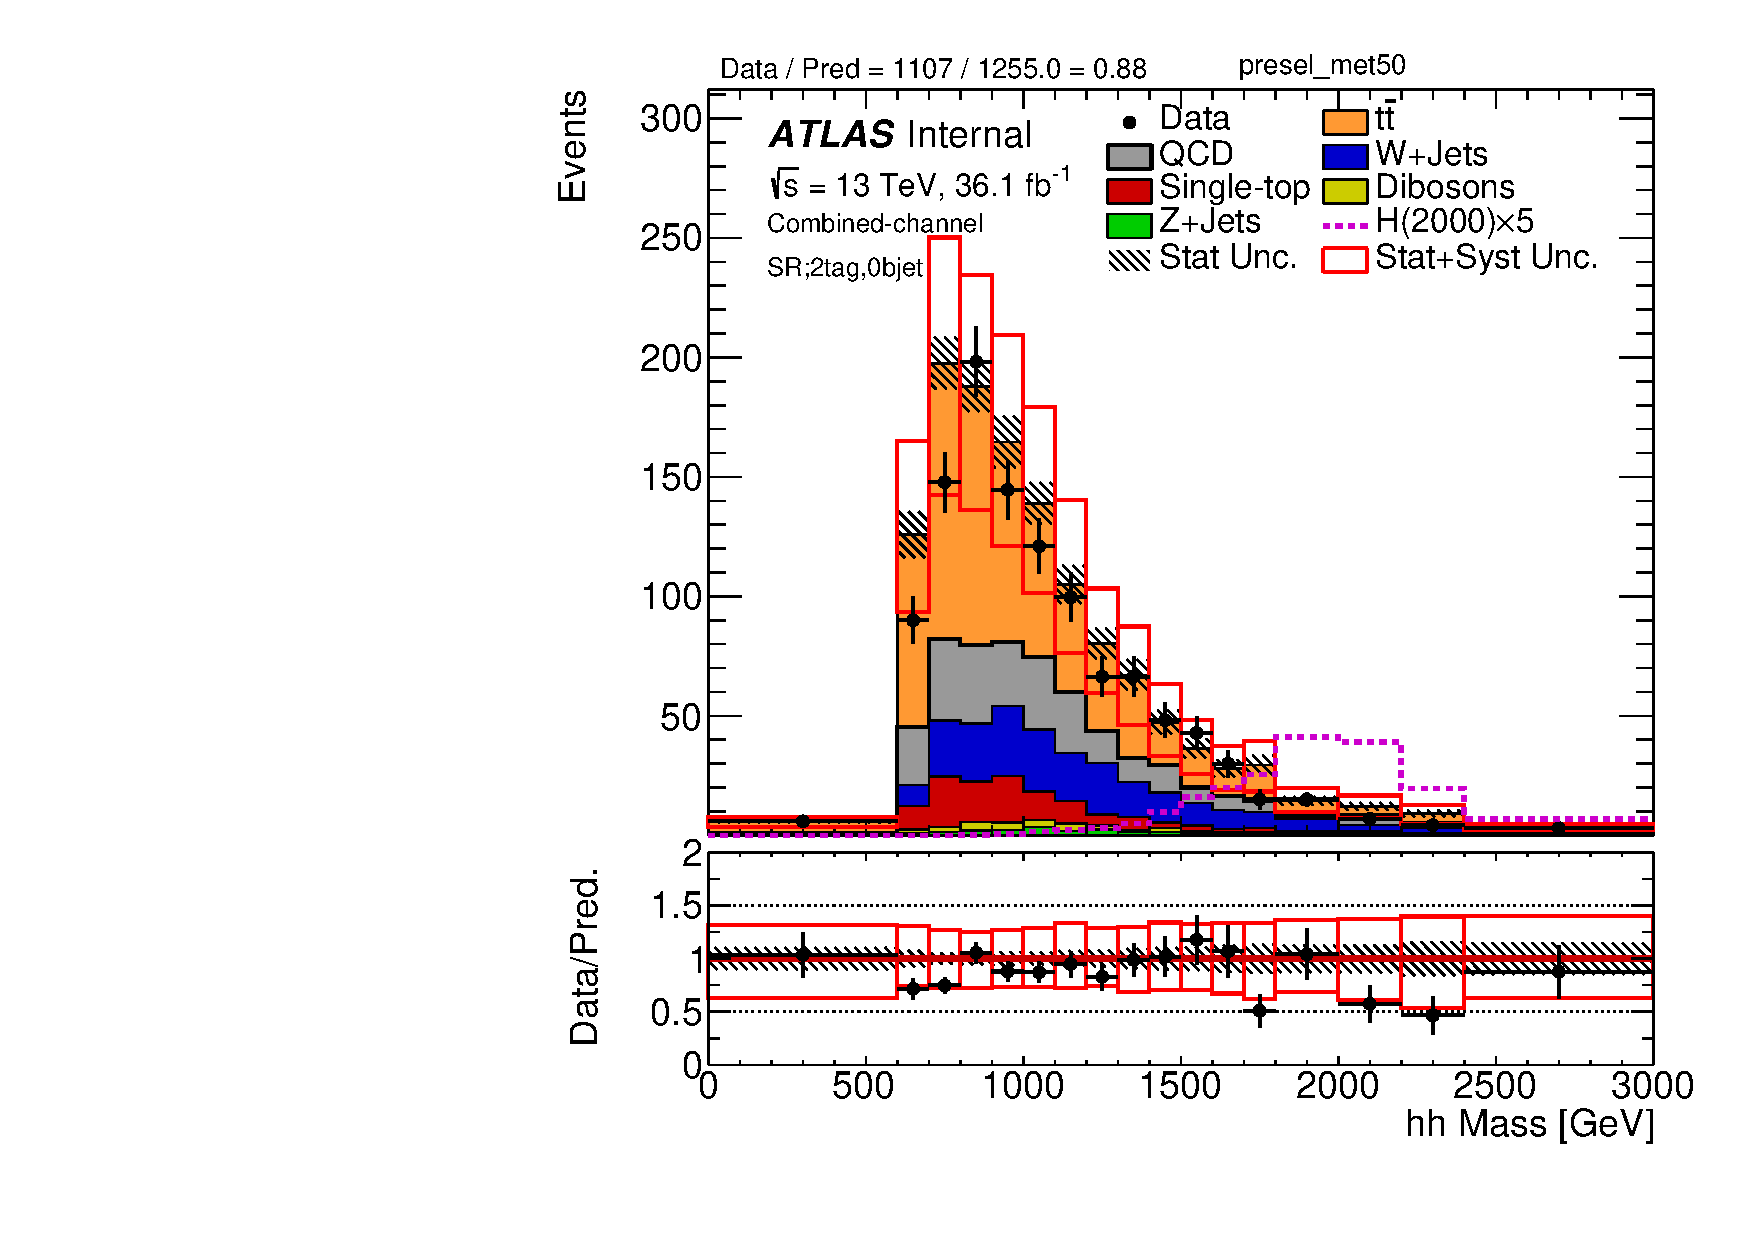
\includegraphics[scale=0.33]{./figures/boosted/PlotsInMbbSR/Unblinded/DataMC_2tag_0bjet_SR_lepton_presel_met50_hhMassRebin1} \\
\par\medskip
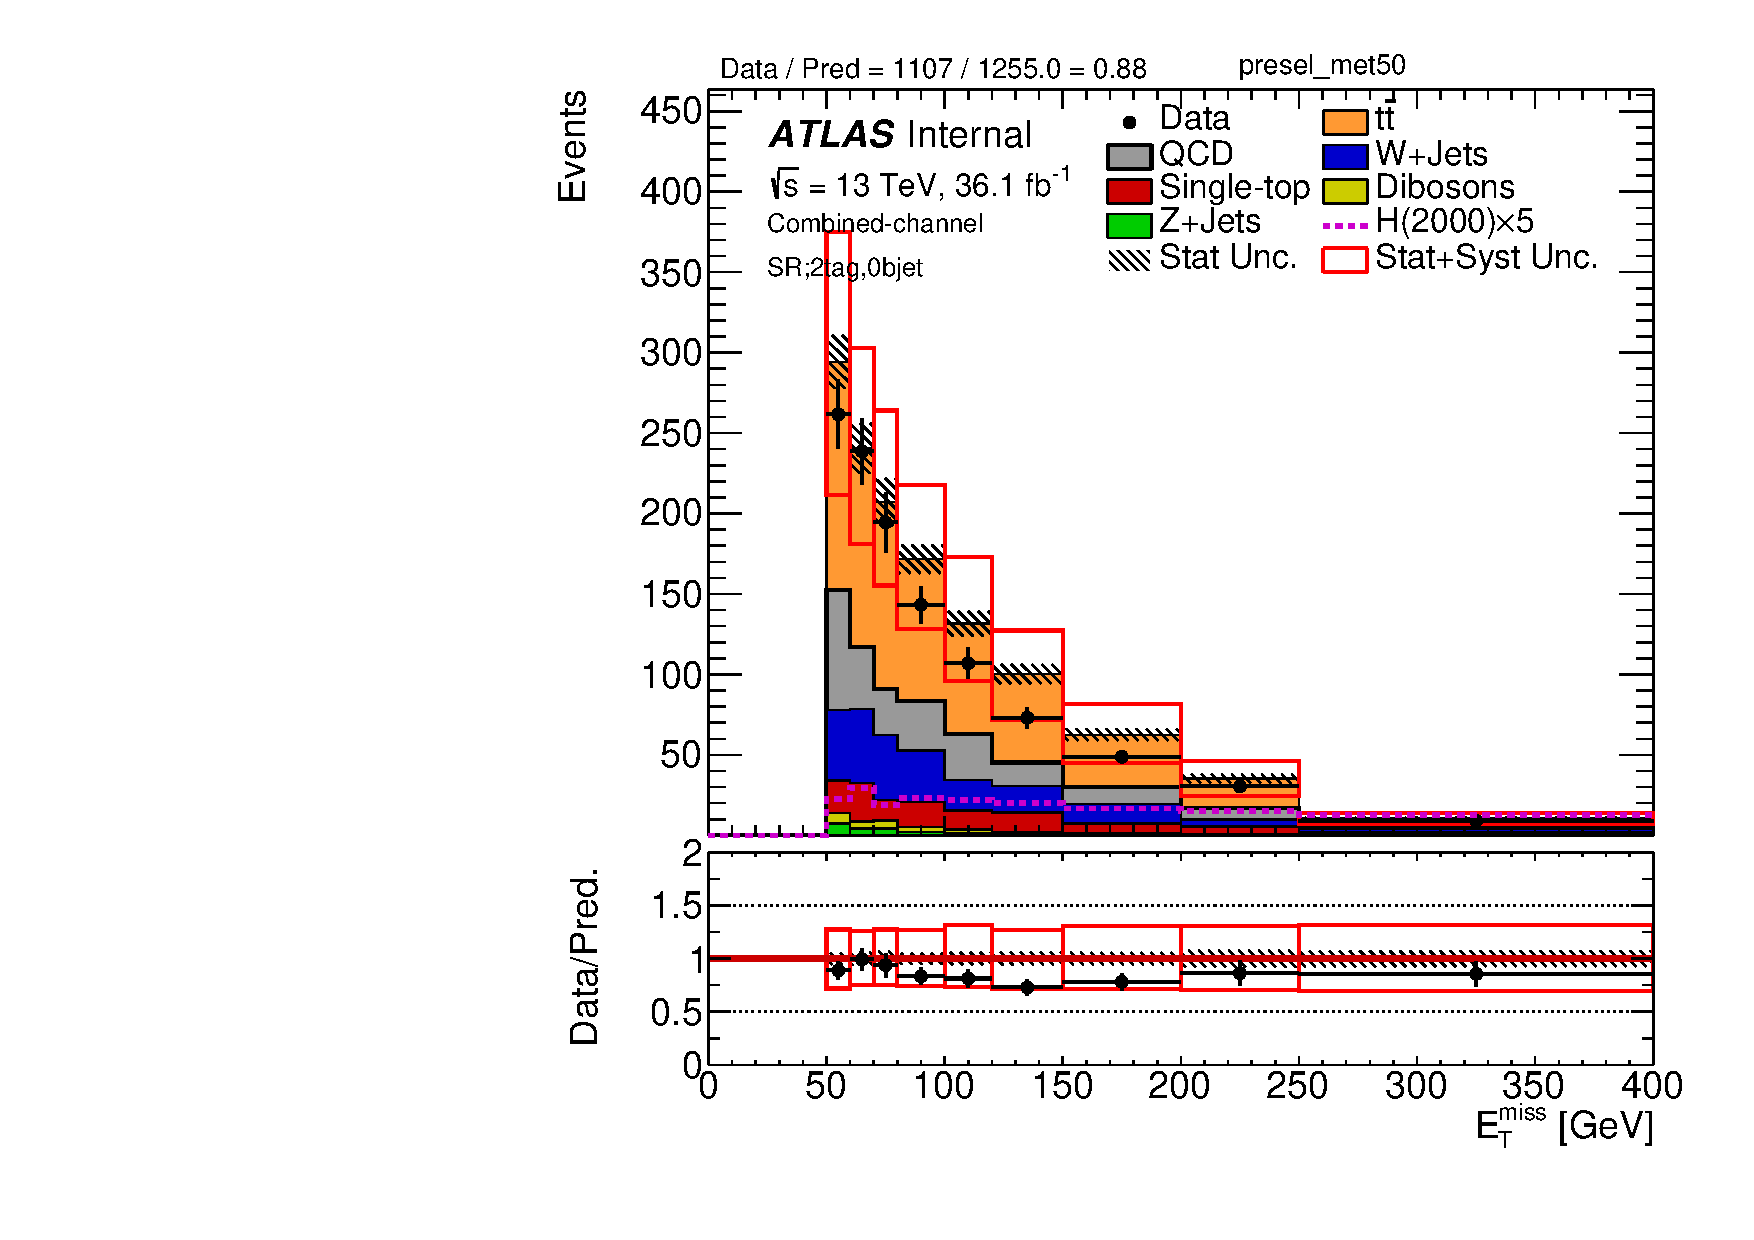
\includegraphics[scale=0.33]{./figures/boosted/PlotsInMbbSR/Unblinded/DataMC_2tag_0bjet_SR_lepton_presel_met50_MET}
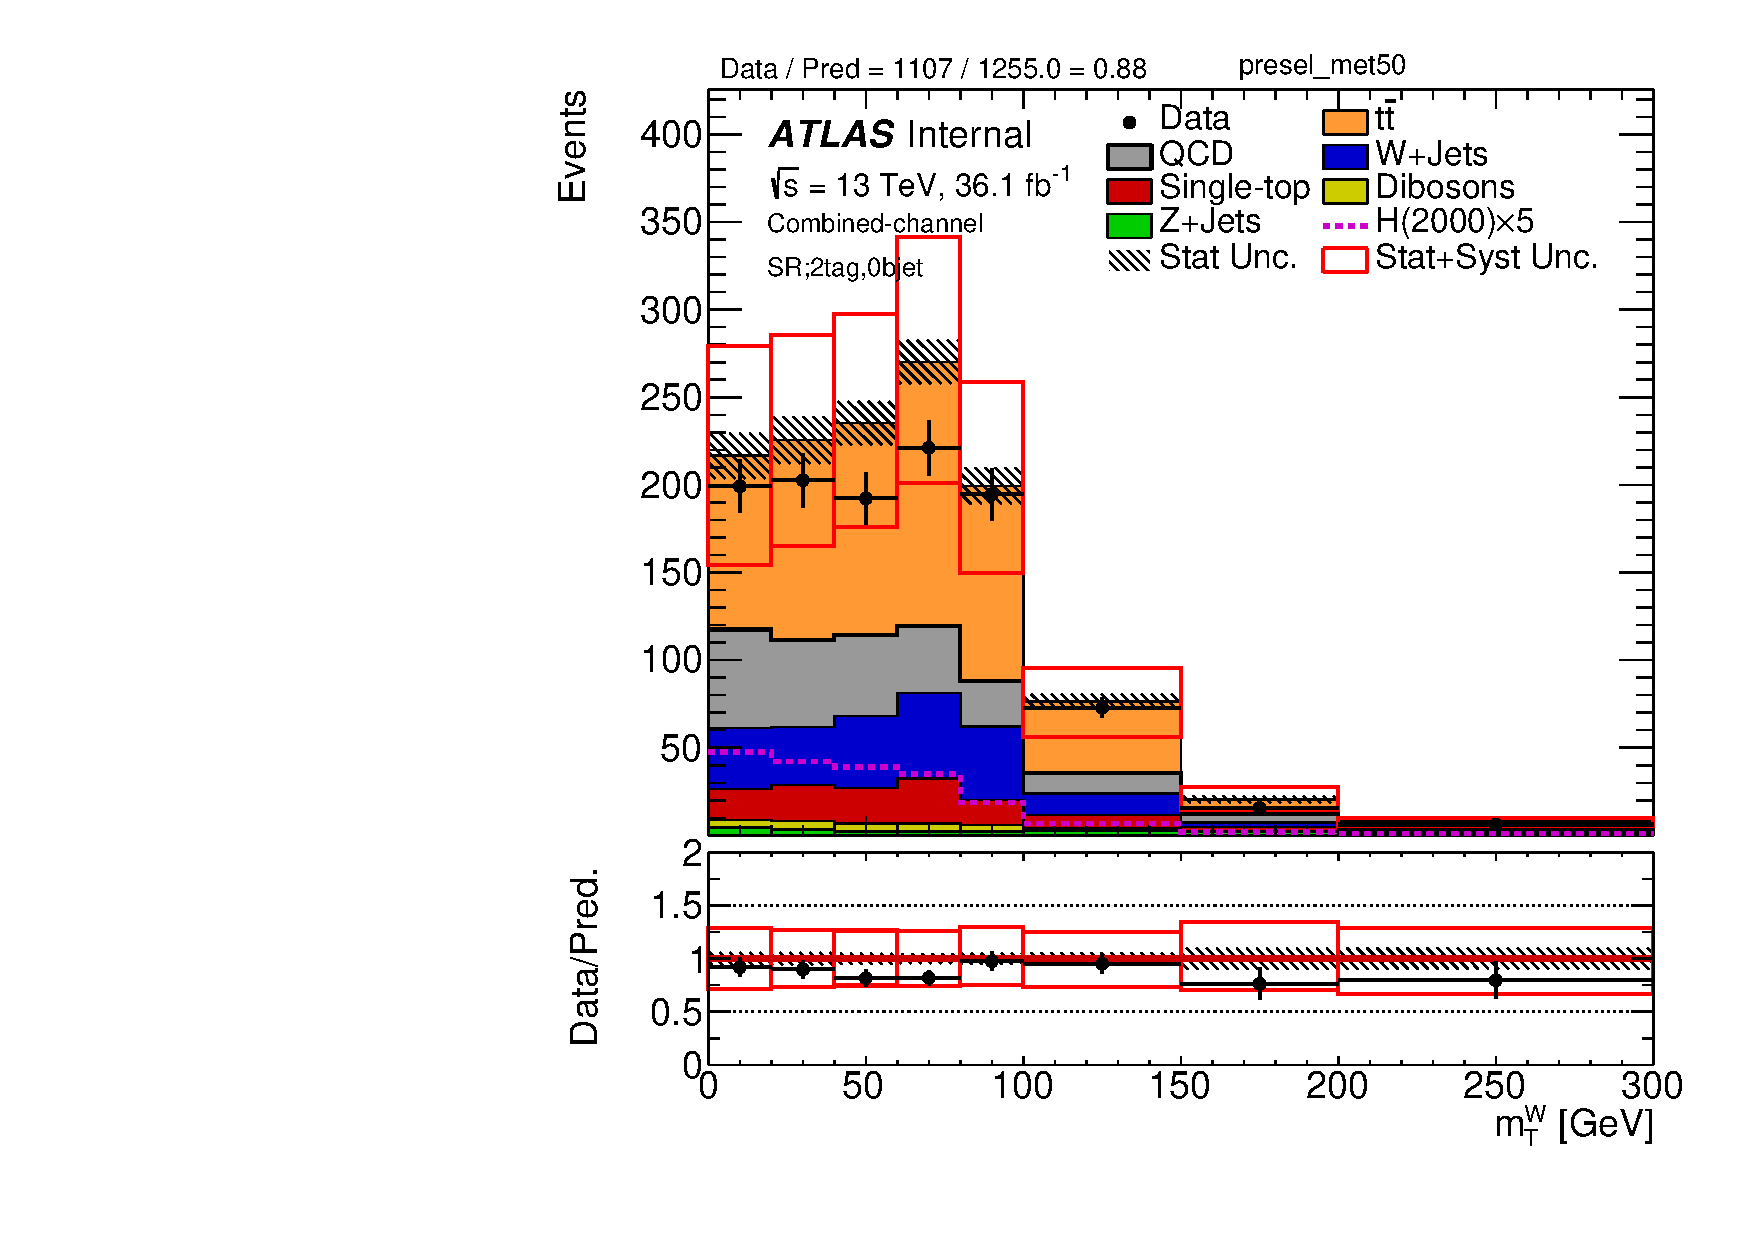
\includegraphics[scale=0.33]{./figures/boosted/PlotsInMbbSR/Unblinded/DataMC_2tag_0bjet_SR_lepton_presel_met50_WlepMtATLAS}
\caption{The invariant mass of the reconstructed di-Higgs (hh) system, \met and transverse mass of the $W \to l\nu$ system 
distributions of events in the signal region (SR).}
\label{fig:boosted_SR_mainplots}
\end{center}
\end{figure}

\begin{figure}[!h]
\begin{center}
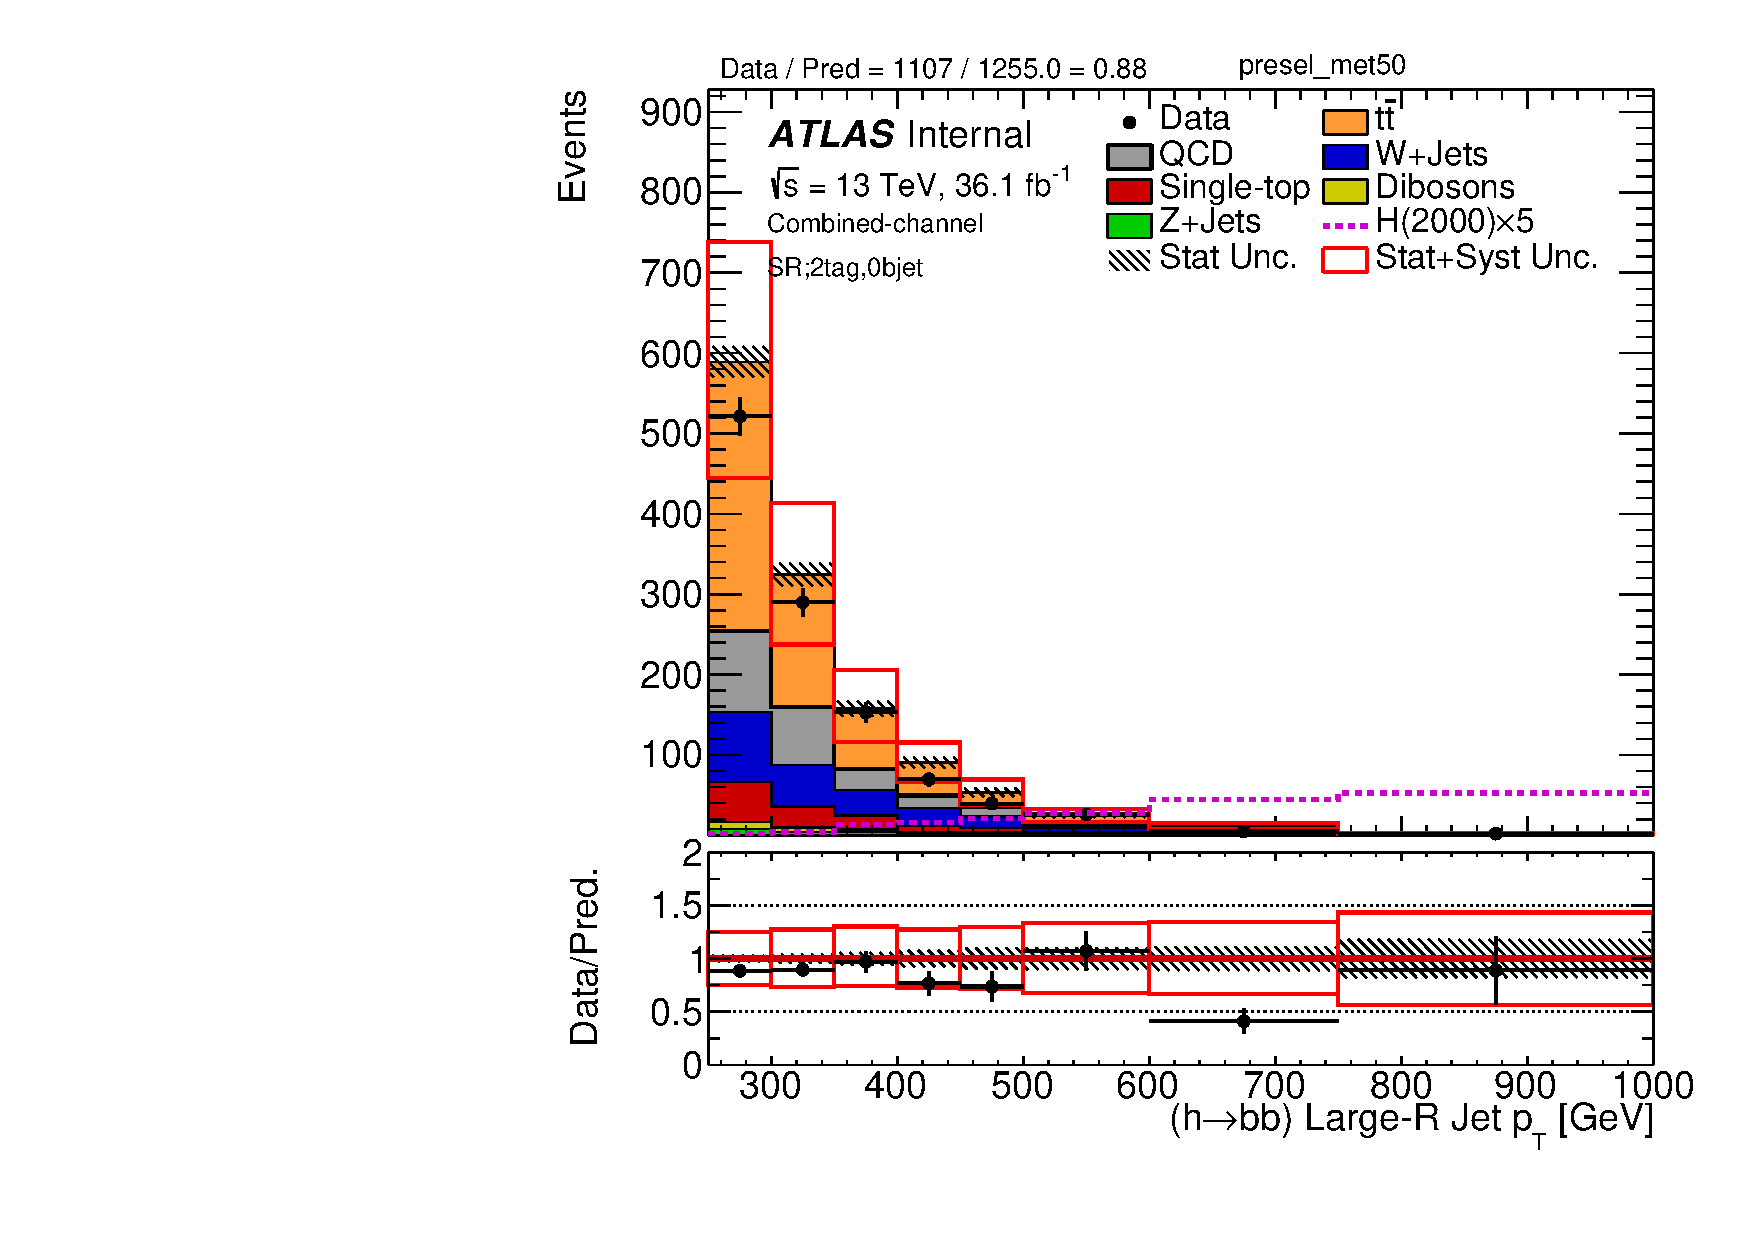
\includegraphics[scale=0.33]{./figures/boosted/PlotsInMbbSR/Unblinded/DataMC_2tag_0bjet_SR_lepton_presel_met50_HbbPt}
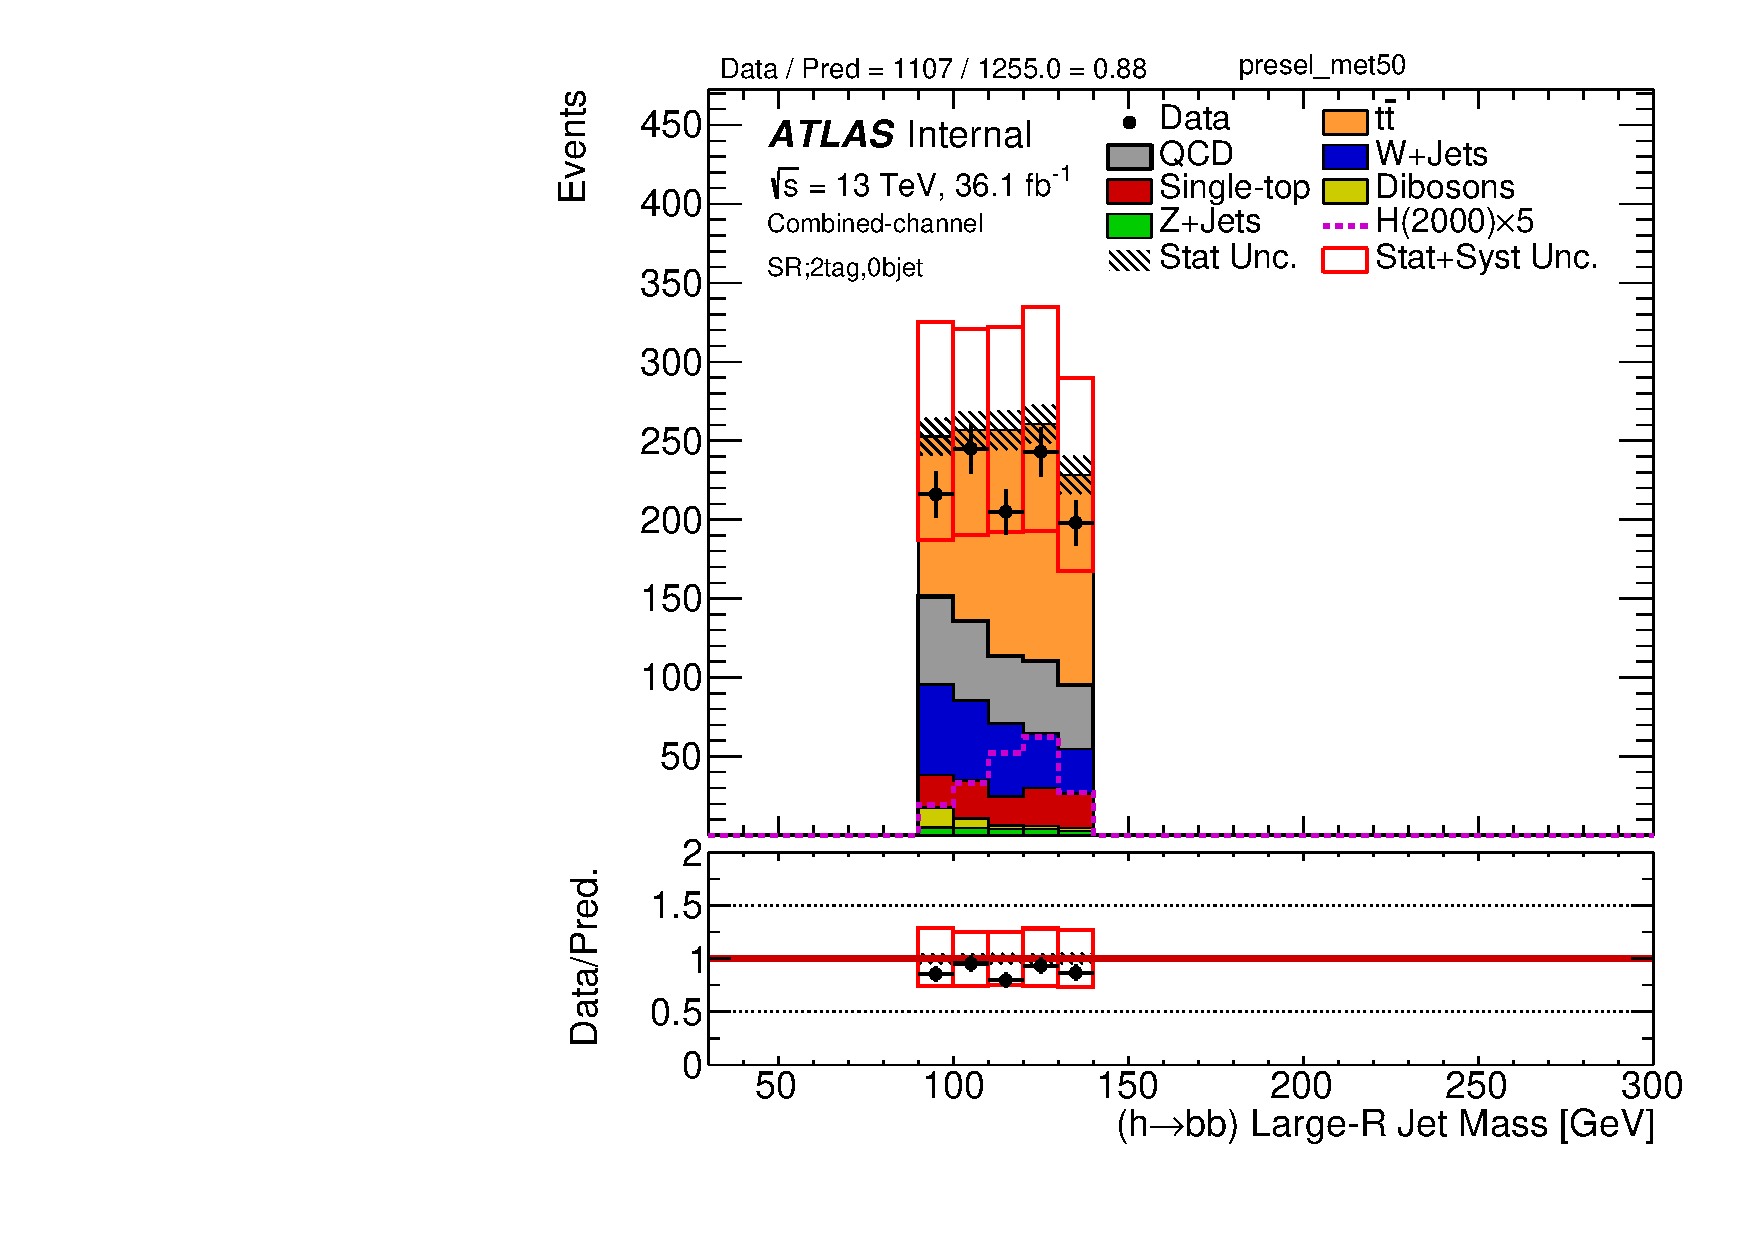
\includegraphics[scale=0.33]{./figures/boosted/PlotsInMbbSR/Unblinded/DataMC_2tag_0bjet_SR_lepton_presel_met50_HbbMass}\\
\par\medskip
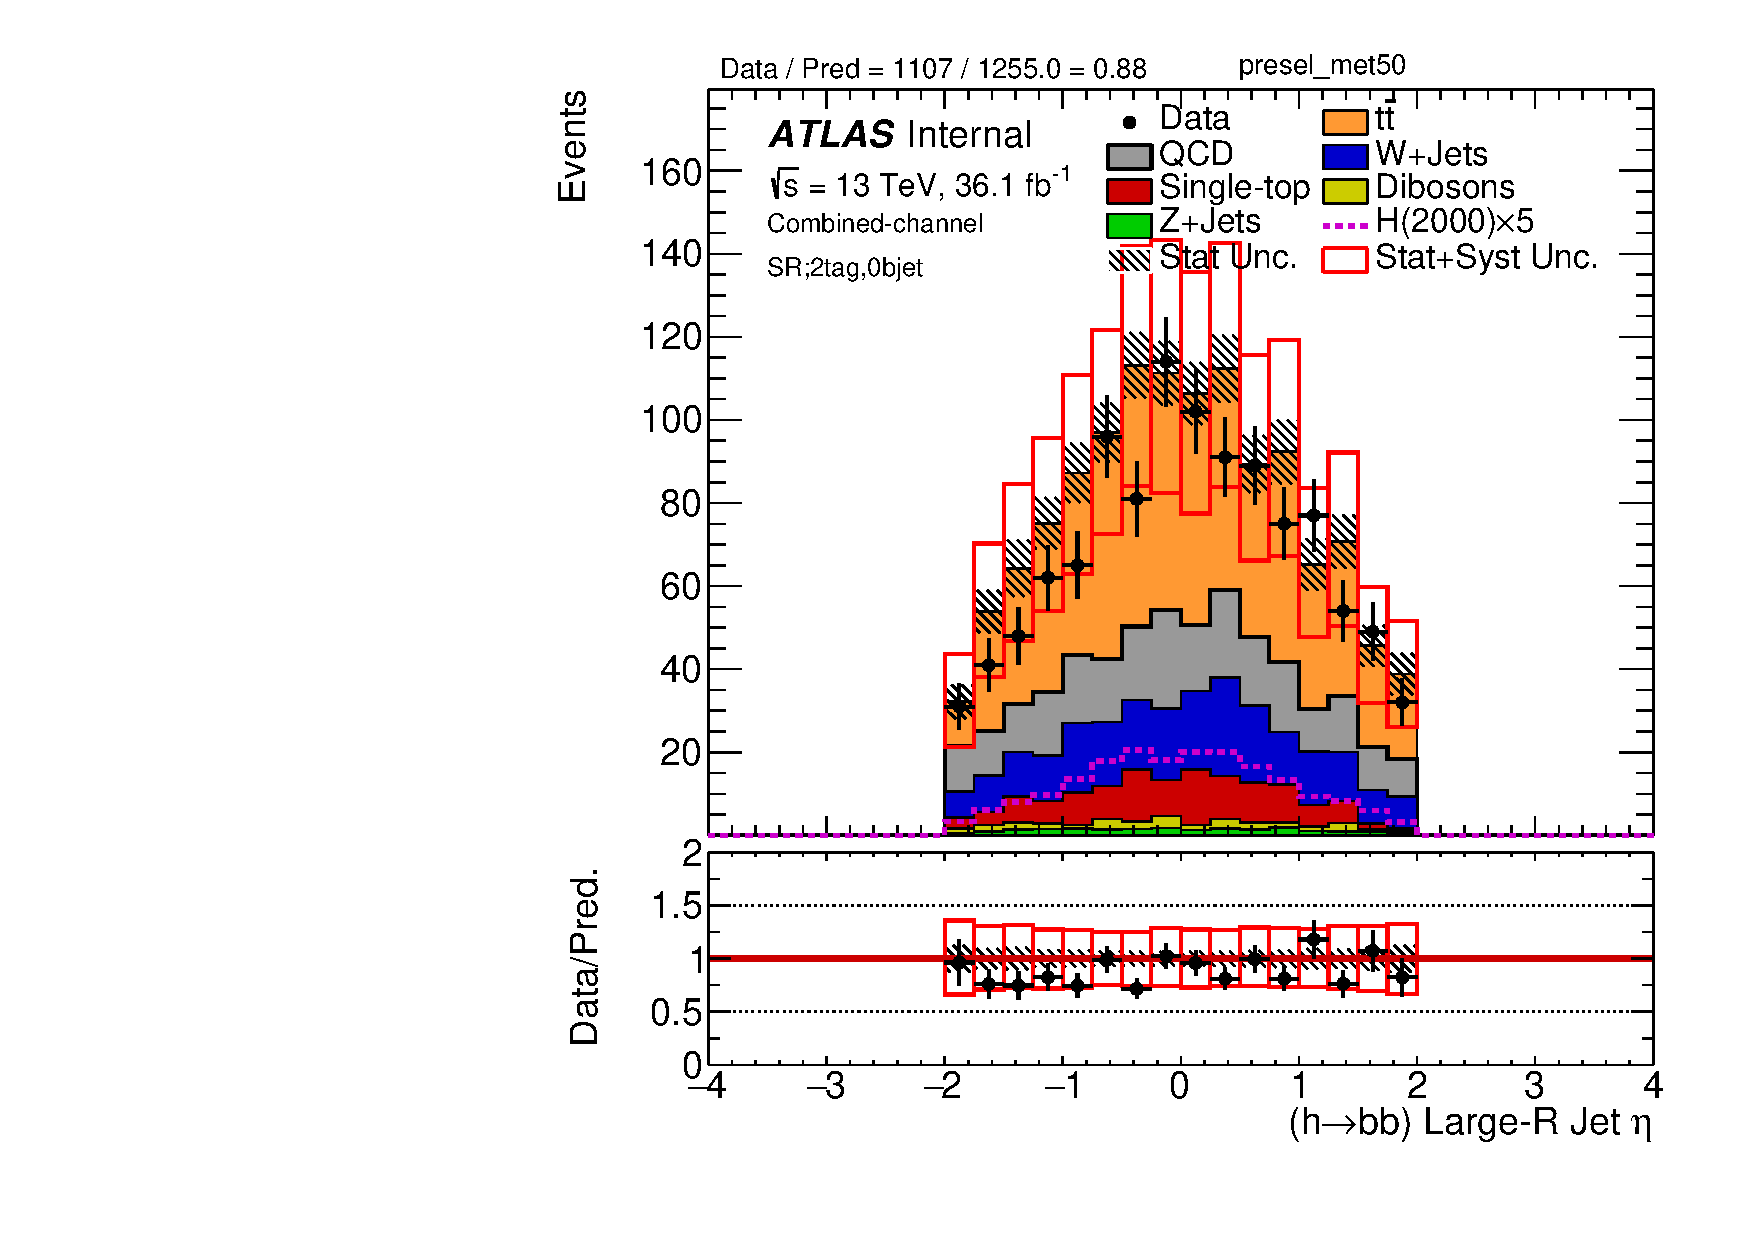
\includegraphics[scale=0.33]{./figures/boosted/PlotsInMbbSR/Unblinded/DataMC_2tag_0bjet_SR_lepton_presel_met50_HbbEta} 
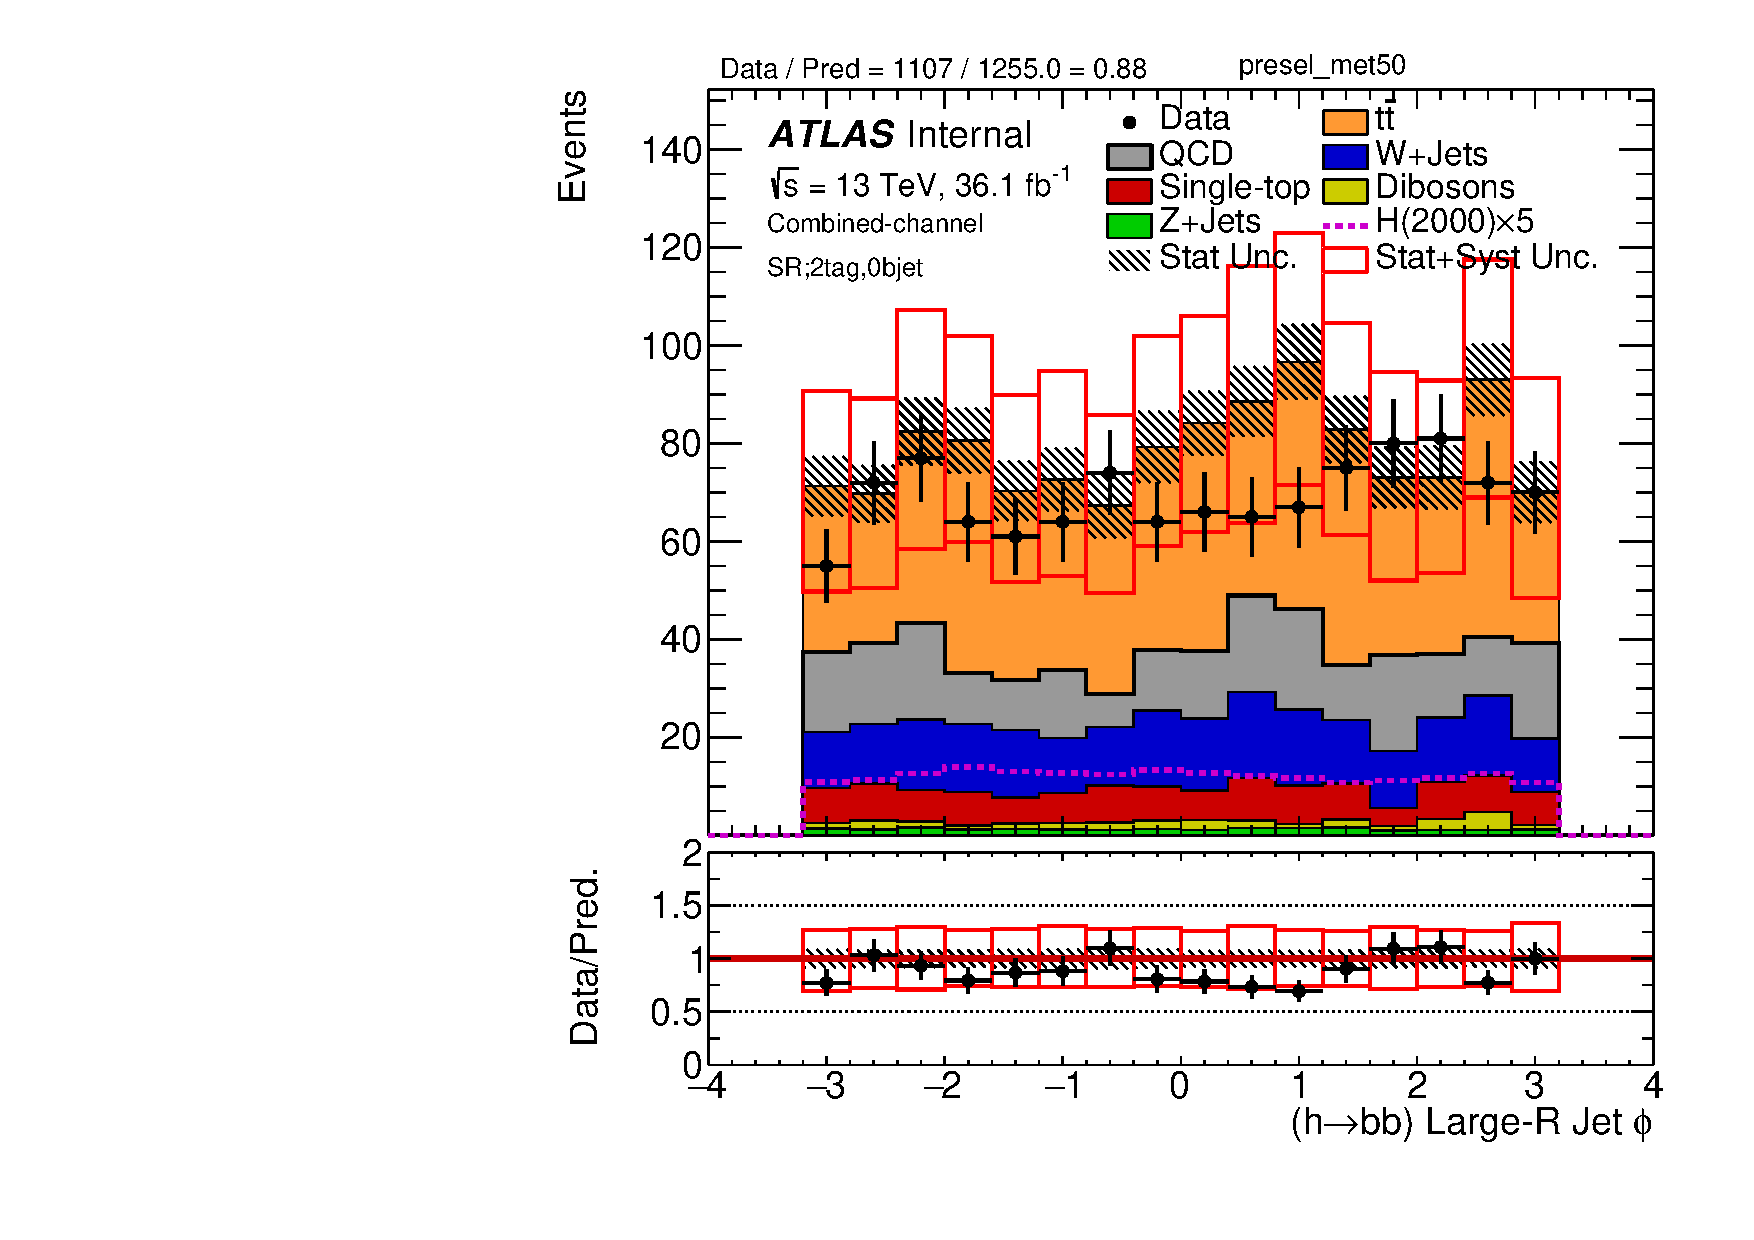
\includegraphics[scale=0.33]{./figures/boosted/PlotsInMbbSR/Unblinded/DataMC_2tag_0bjet_SR_lepton_presel_met50_HbbPhi} 
\caption{Kinematic distributions of the reconstructed large-$R$ jet in the signal region (SR).}
\label{fig:boosted_SR_largerjet}
\end{center}
\end{figure}

\begin{figure}[!h]
\begin{center}
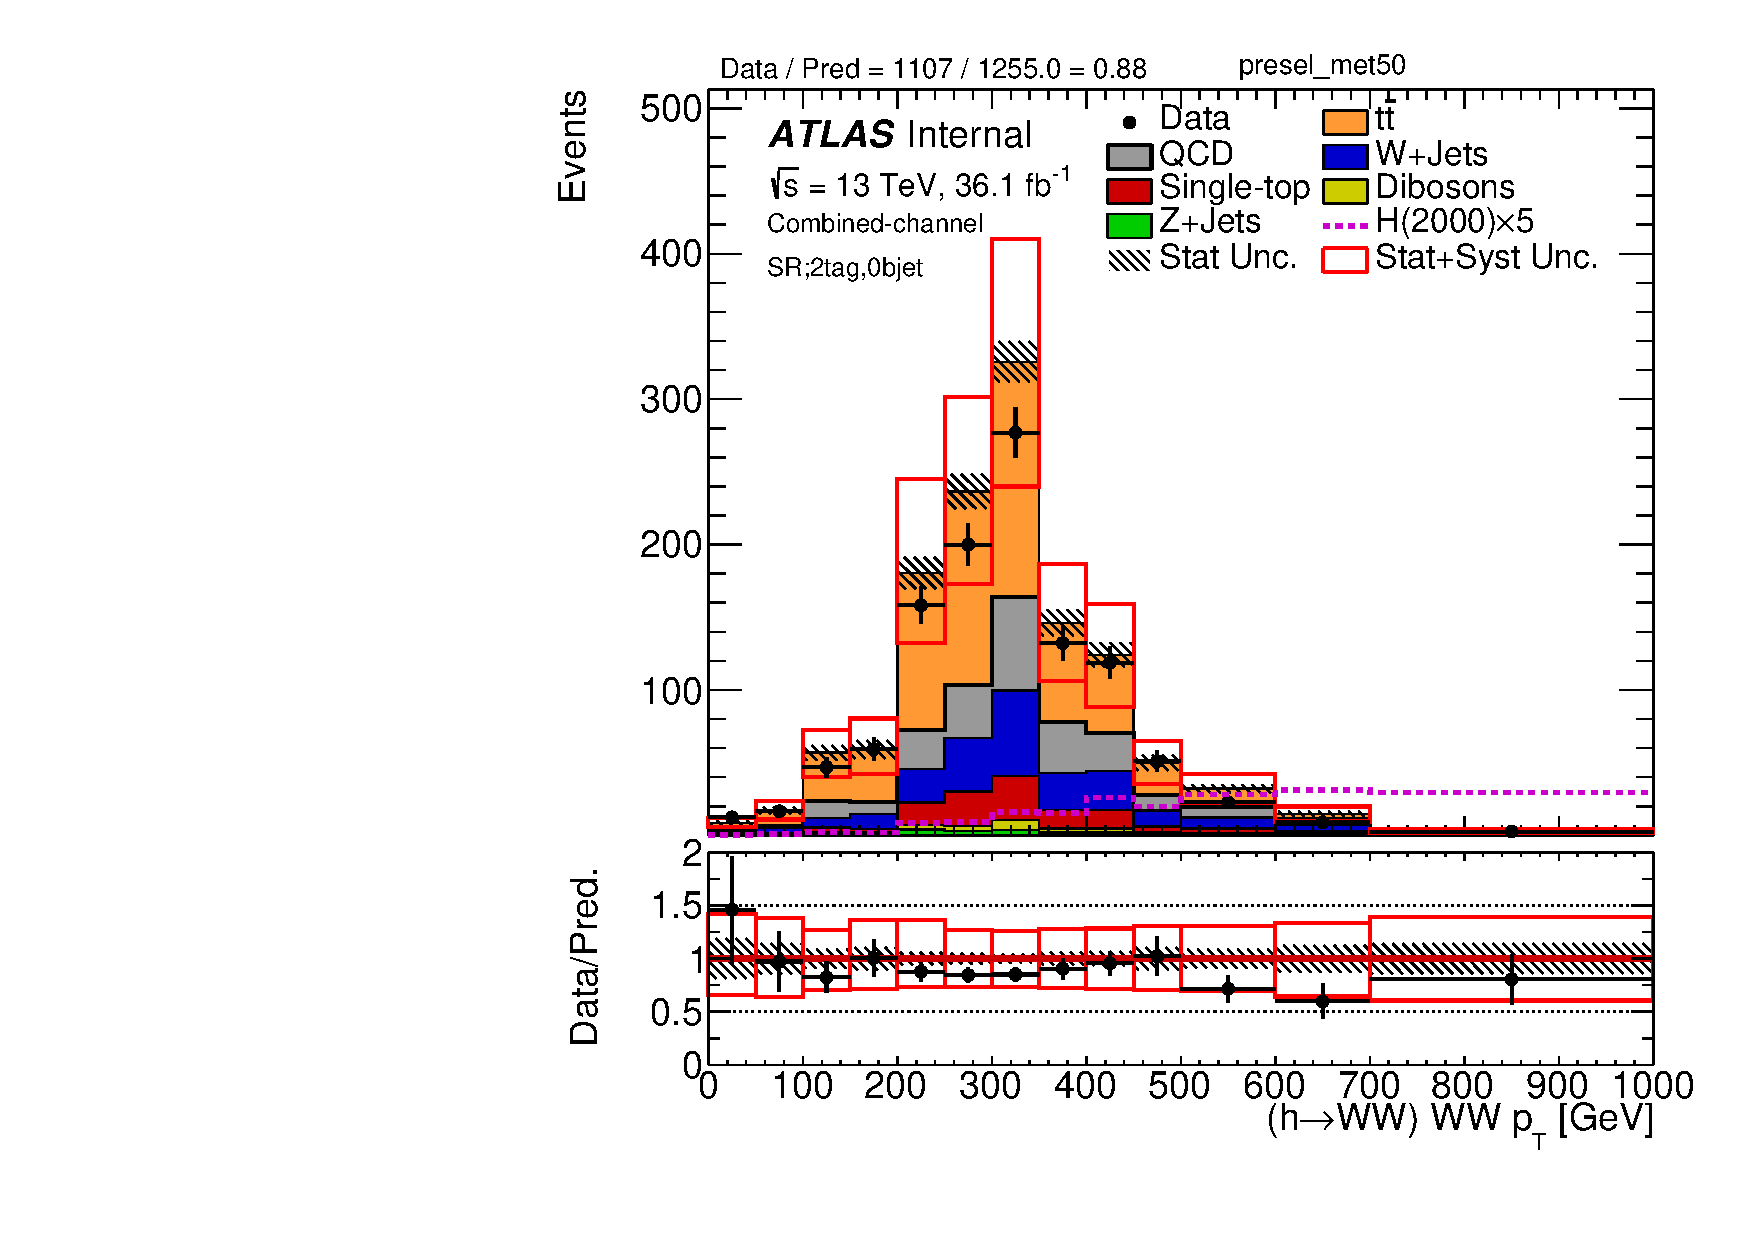
\includegraphics[scale=0.33]{./figures/boosted/PlotsInMbbSR/Unblinded/DataMC_2tag_0bjet_SR_lepton_presel_met50_WWPt}
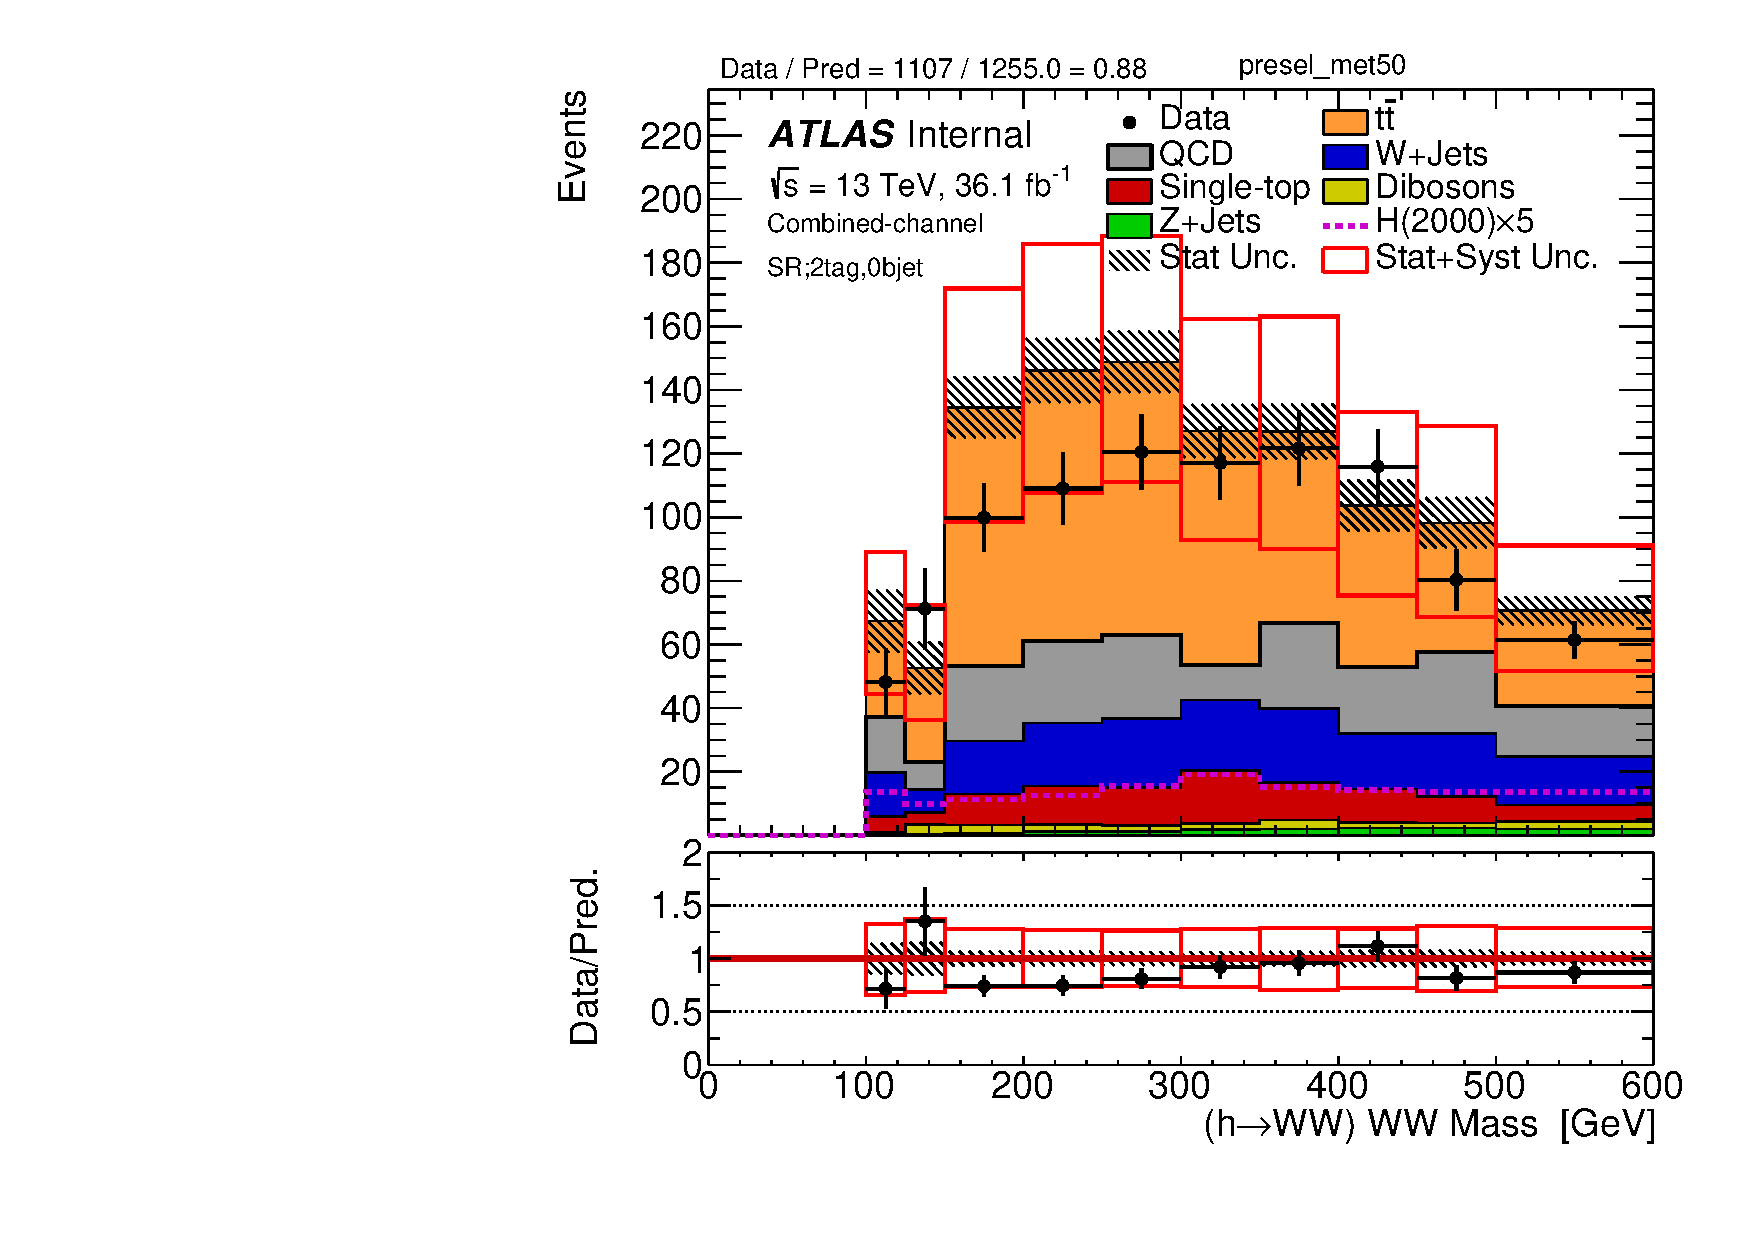
\includegraphics[scale=0.33]{./figures/boosted/PlotsInMbbSR/Unblinded/DataMC_2tag_0bjet_SR_lepton_presel_met50_WWMass}\\
\par\medskip
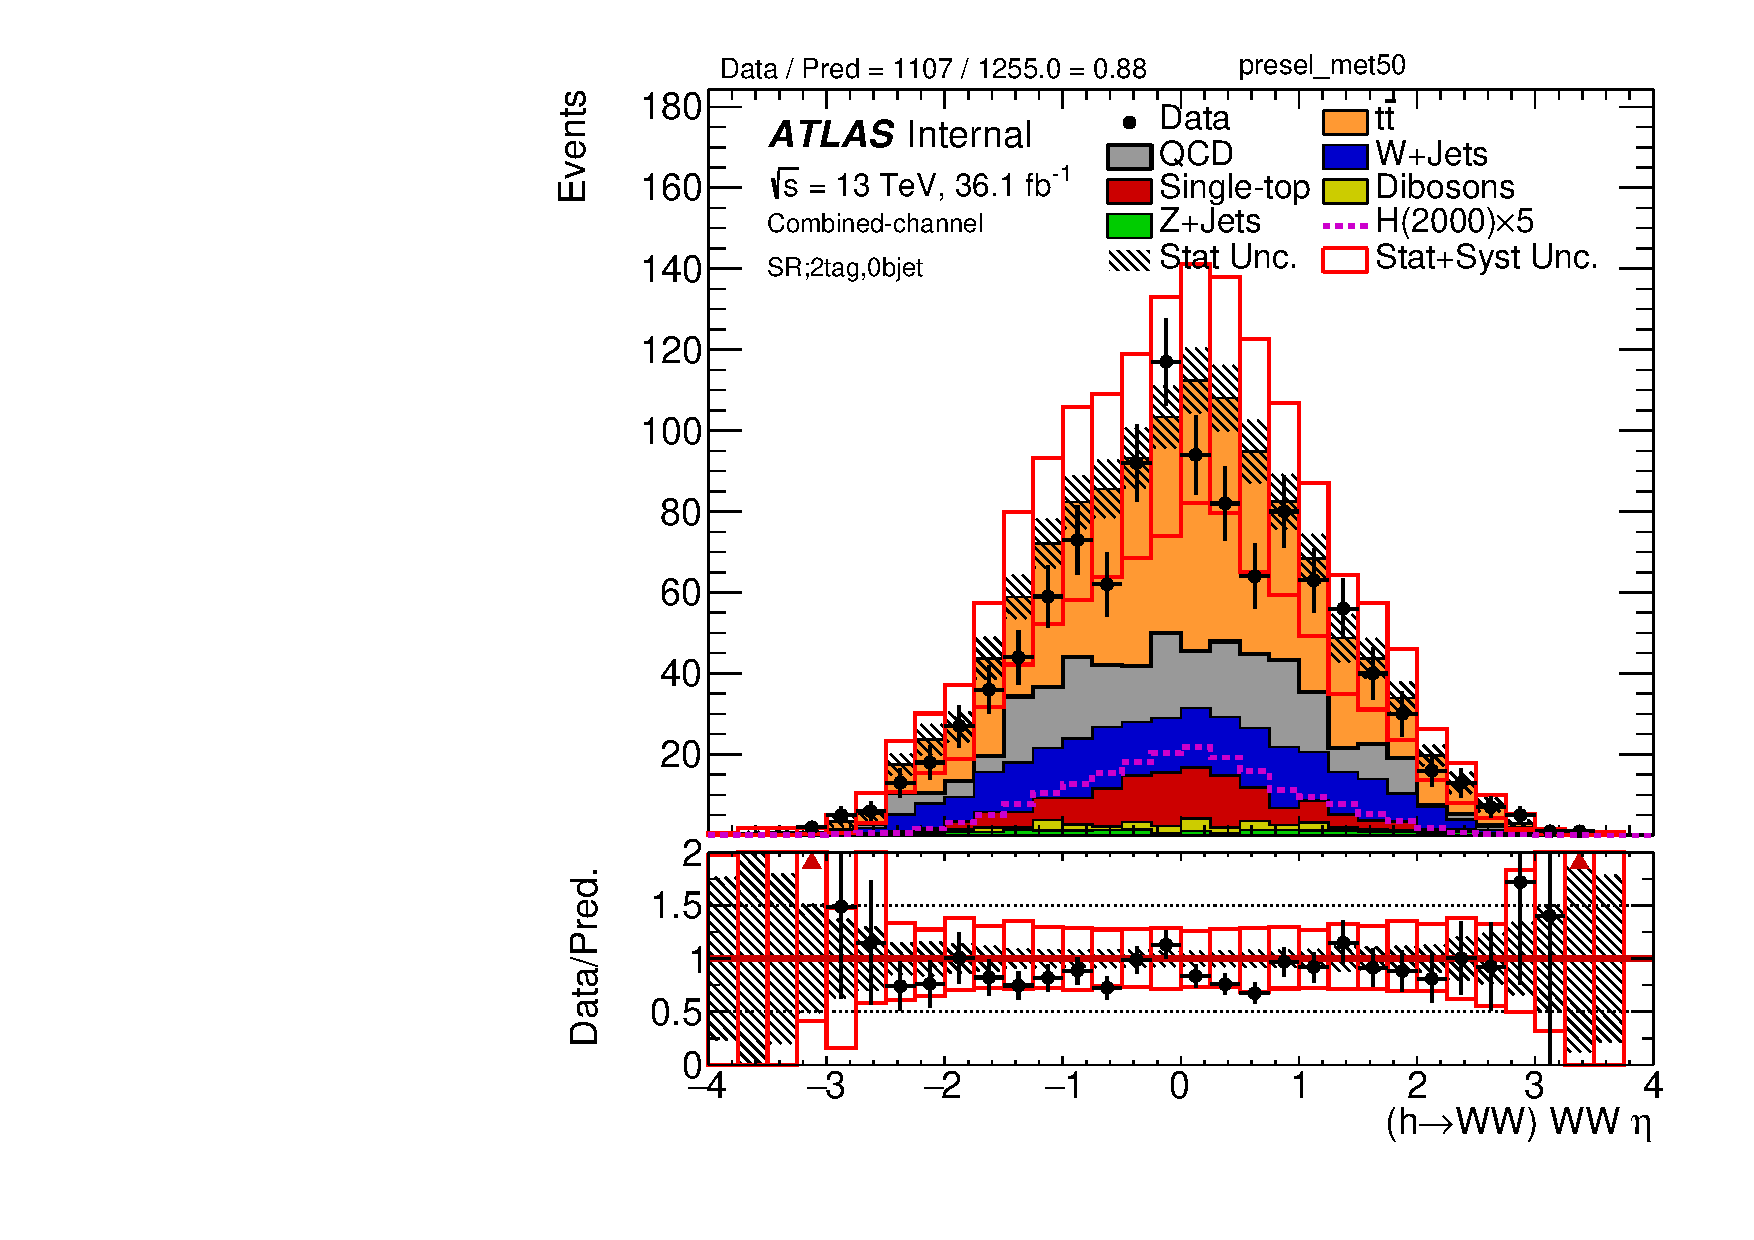
\includegraphics[scale=0.33]{./figures/boosted/PlotsInMbbSR/Unblinded/DataMC_2tag_0bjet_SR_lepton_presel_met50_WWEta}
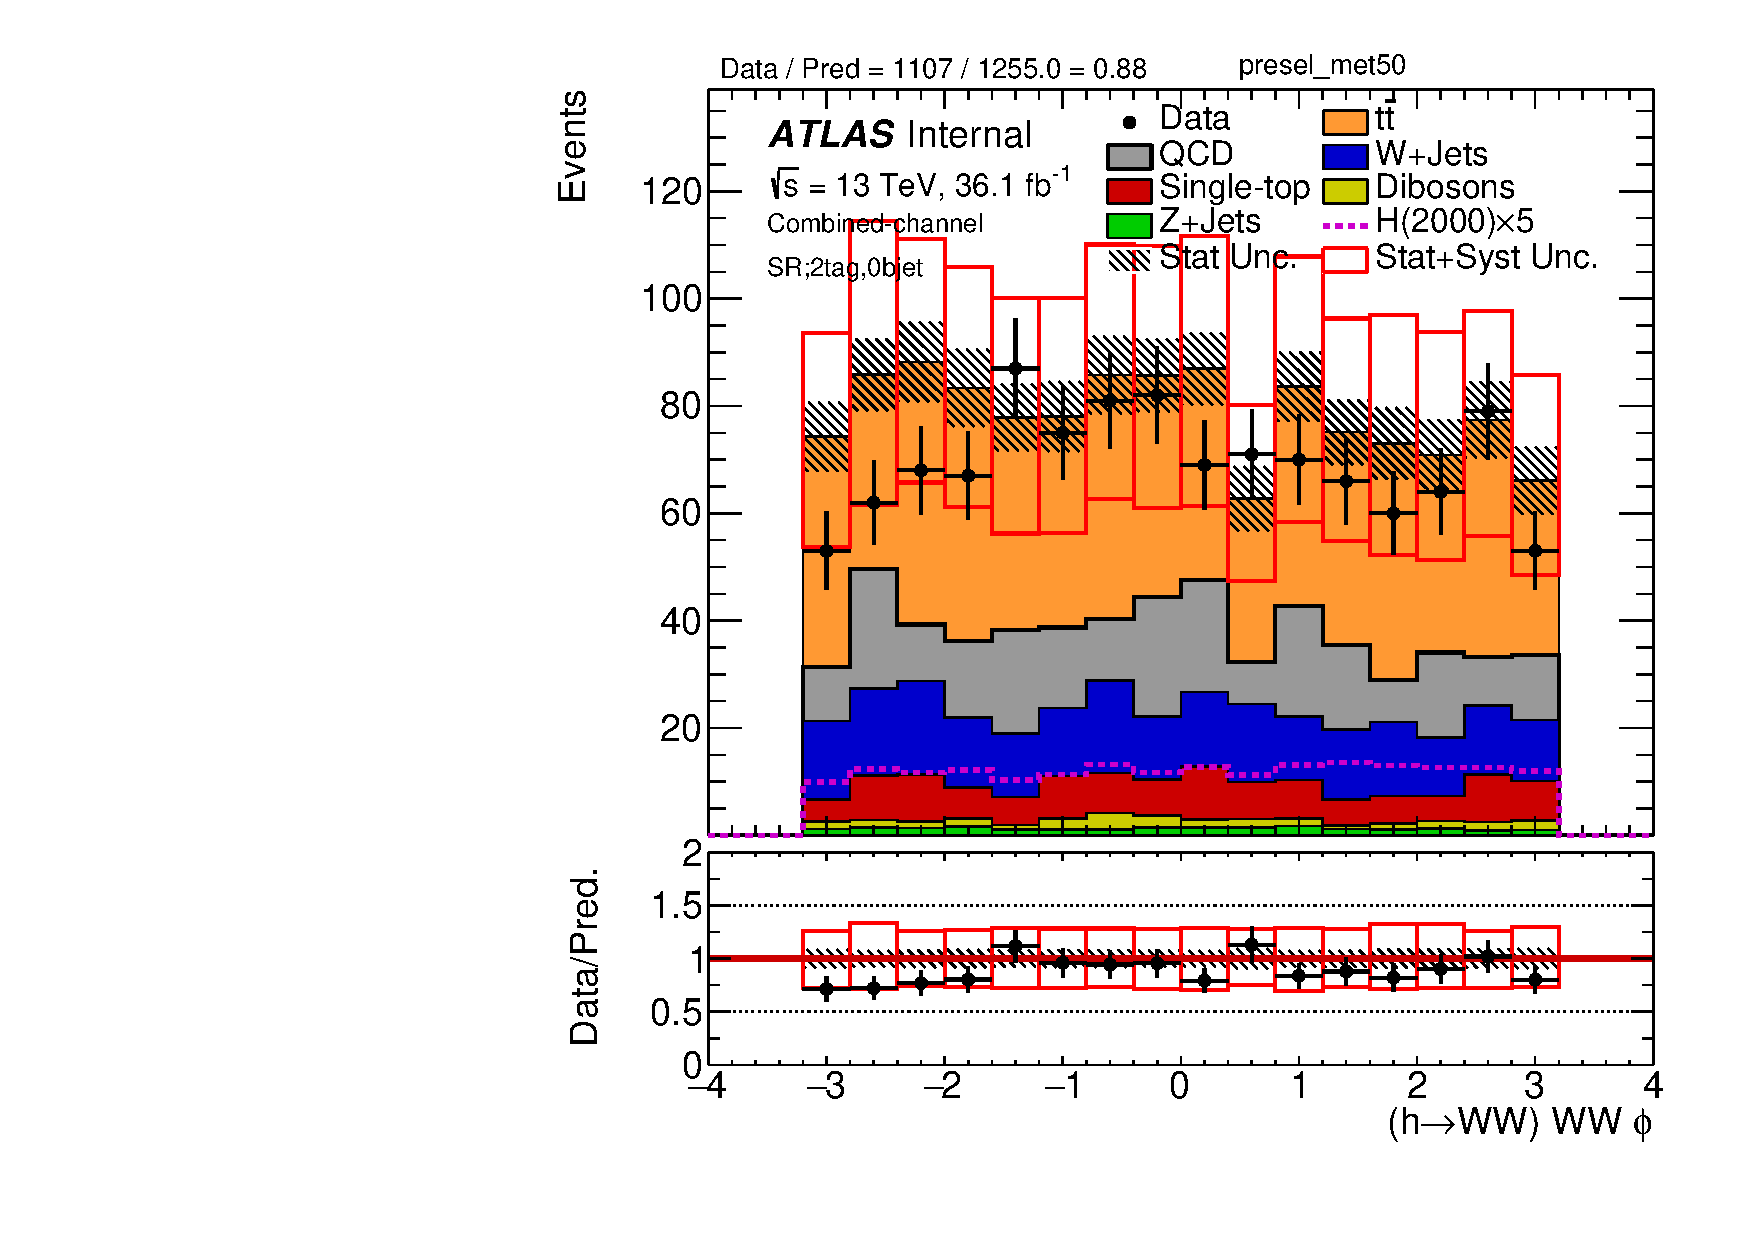
\includegraphics[scale=0.33]{./figures/boosted/PlotsInMbbSR/Unblinded/DataMC_2tag_0bjet_SR_lepton_presel_met50_WWPhi}
\caption{Kinematic distributions of the reconstructed $h \to WW$ system in the signal region (SR).}
\label{fig:boosted_SR_wwsystem}
\end{center}
\end{figure}

\begin{figure}[!h]
\begin{center}
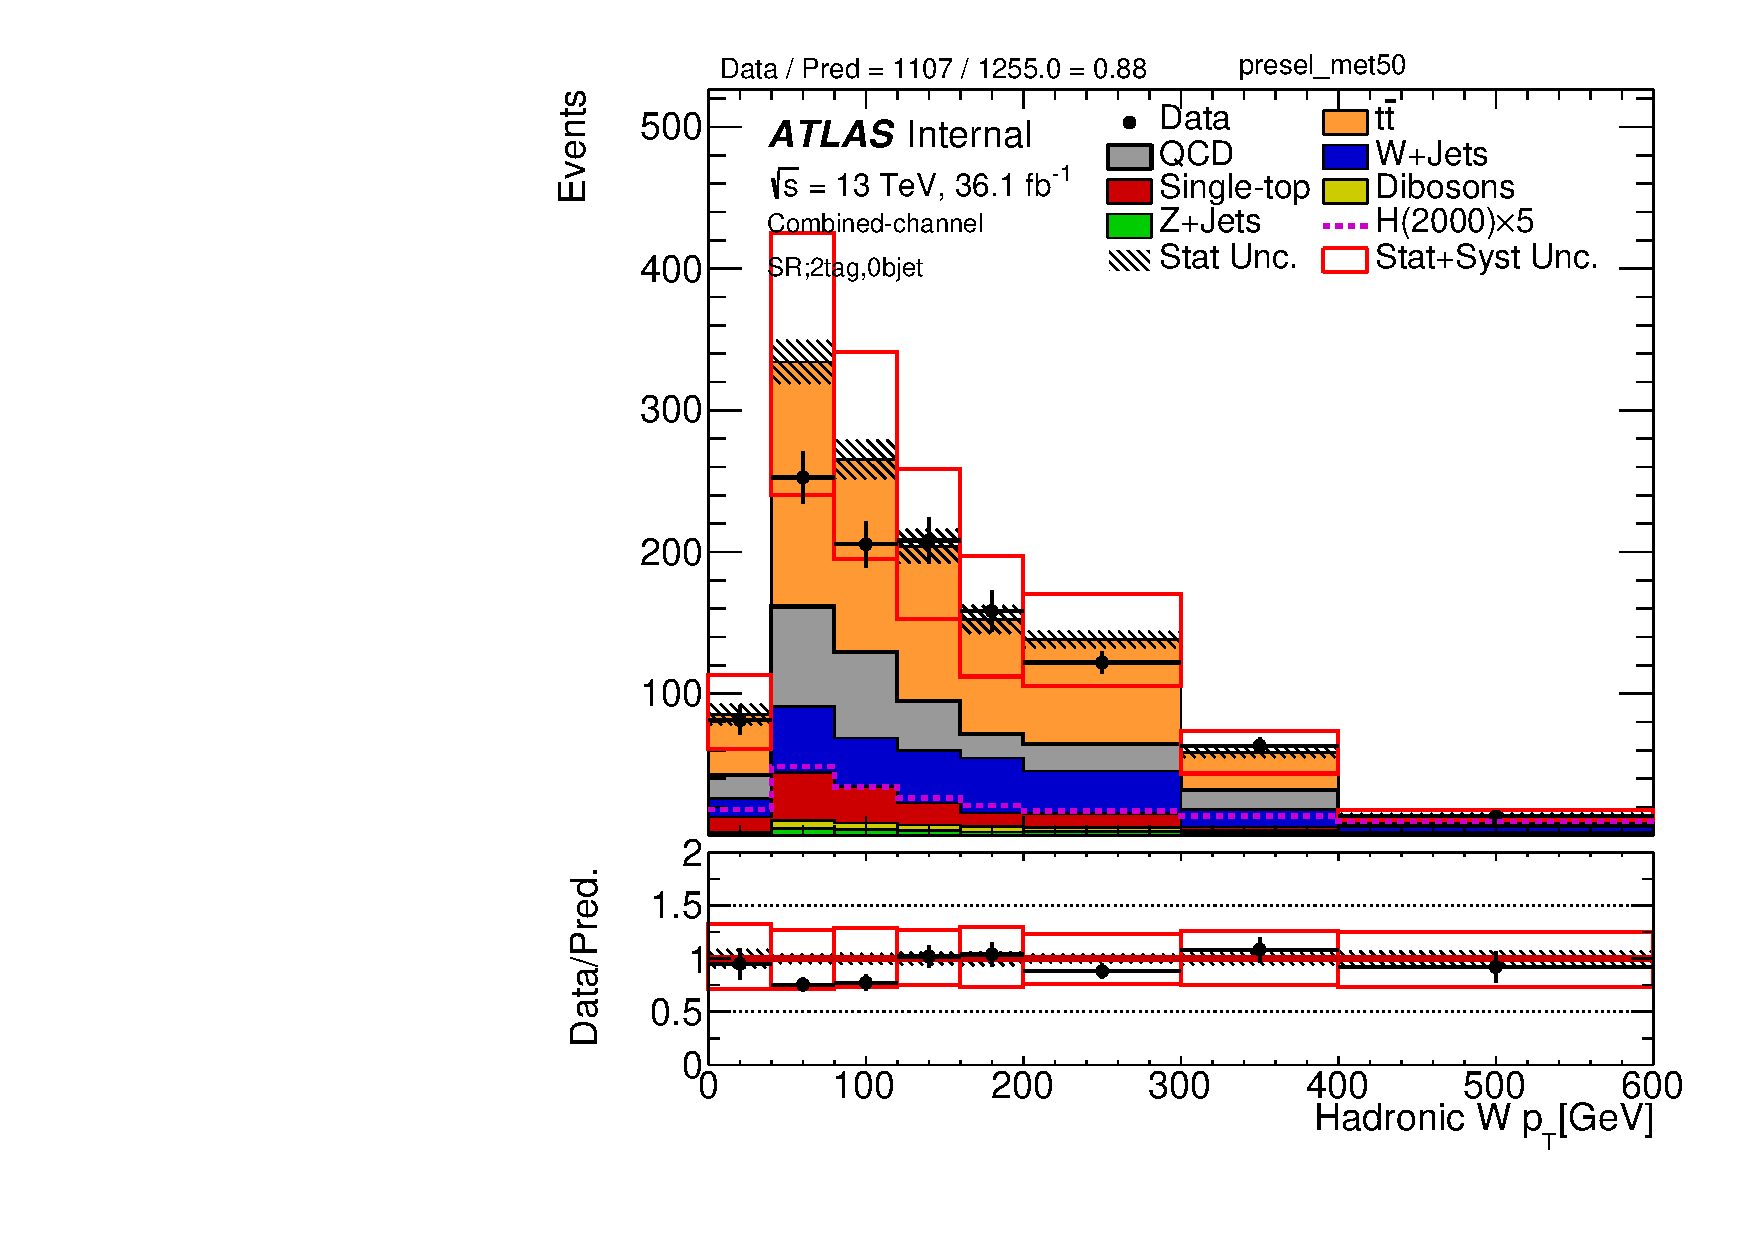
\includegraphics[scale=0.33]{./figures/boosted/PlotsInMbbSR/Unblinded/DataMC_2tag_0bjet_SR_lepton_presel_met50_WhadPt}
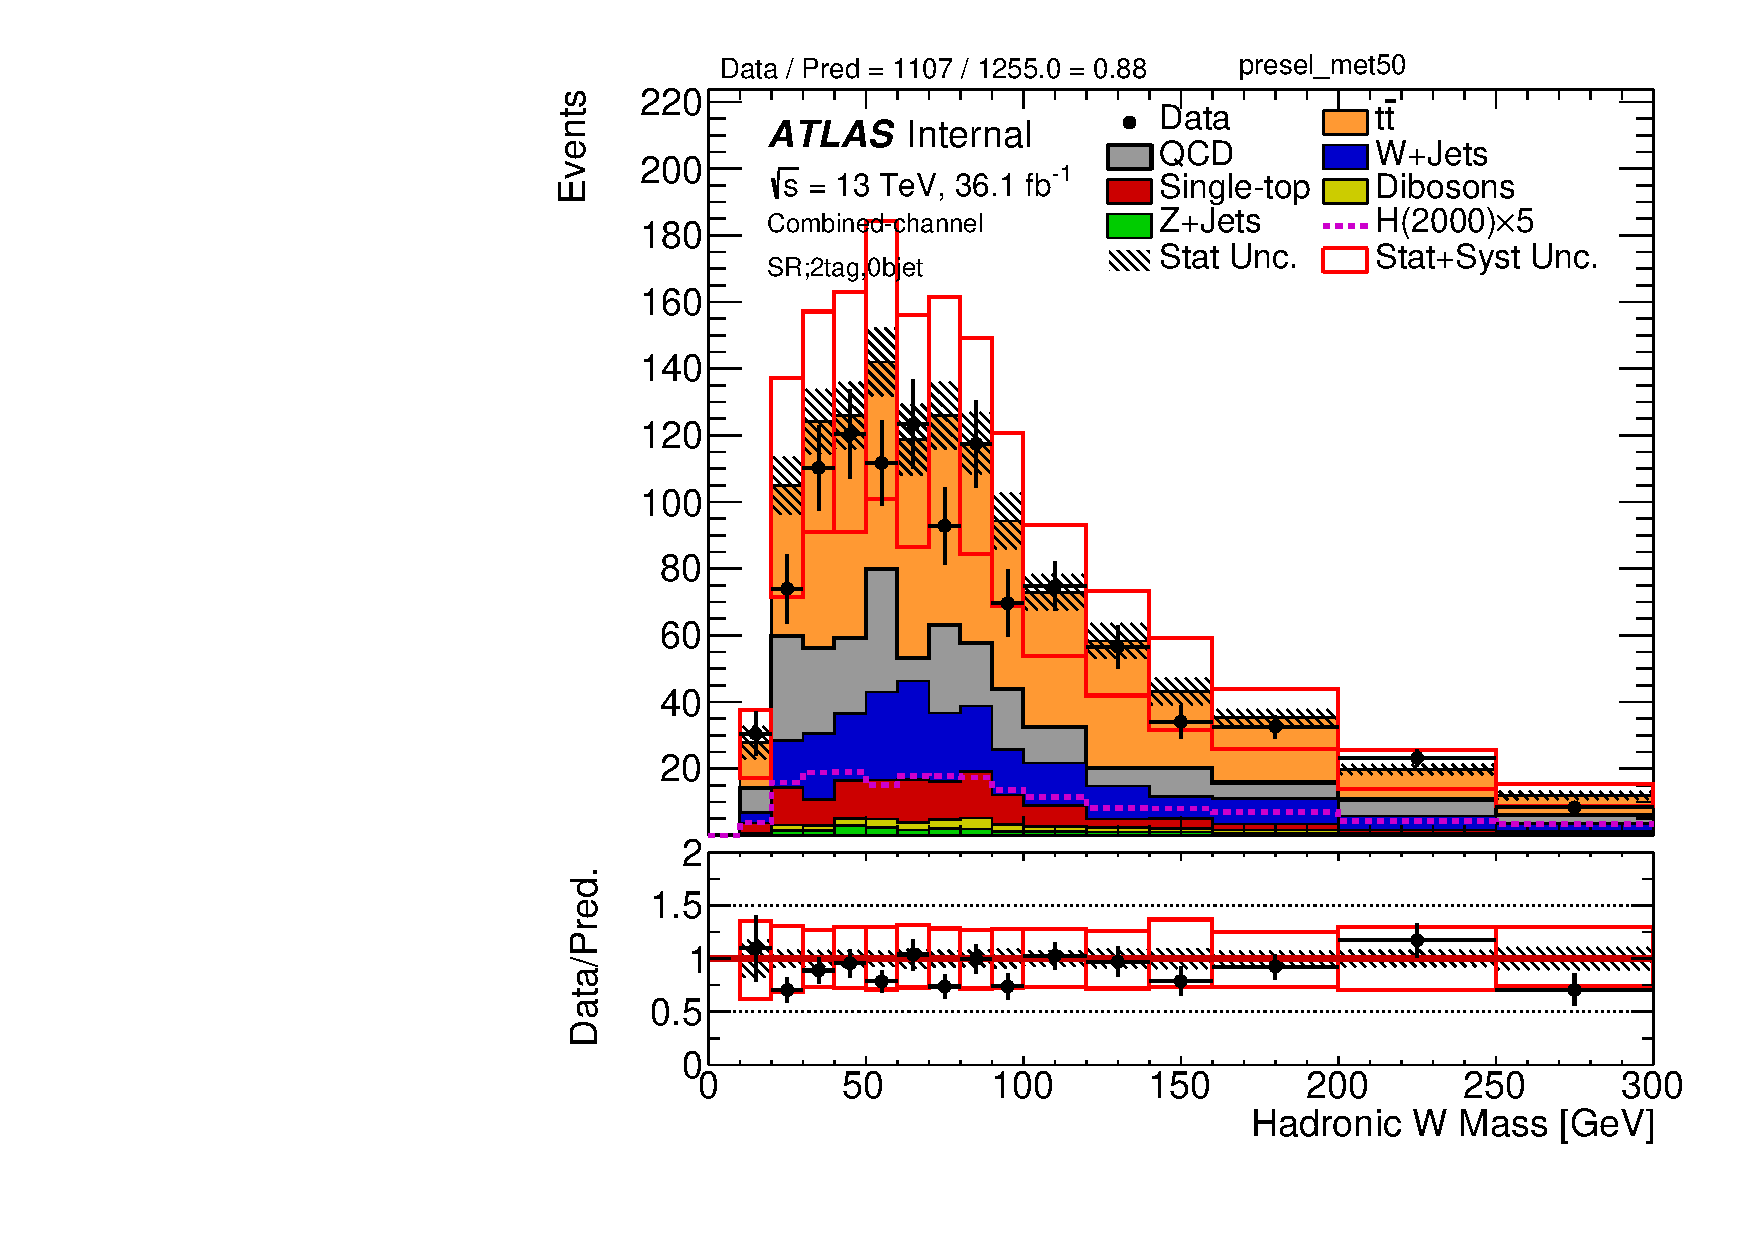
\includegraphics[scale=0.33]{./figures/boosted/PlotsInMbbSR/Unblinded/DataMC_2tag_0bjet_SR_lepton_presel_met50_WhadMass} \\
\par\medskip
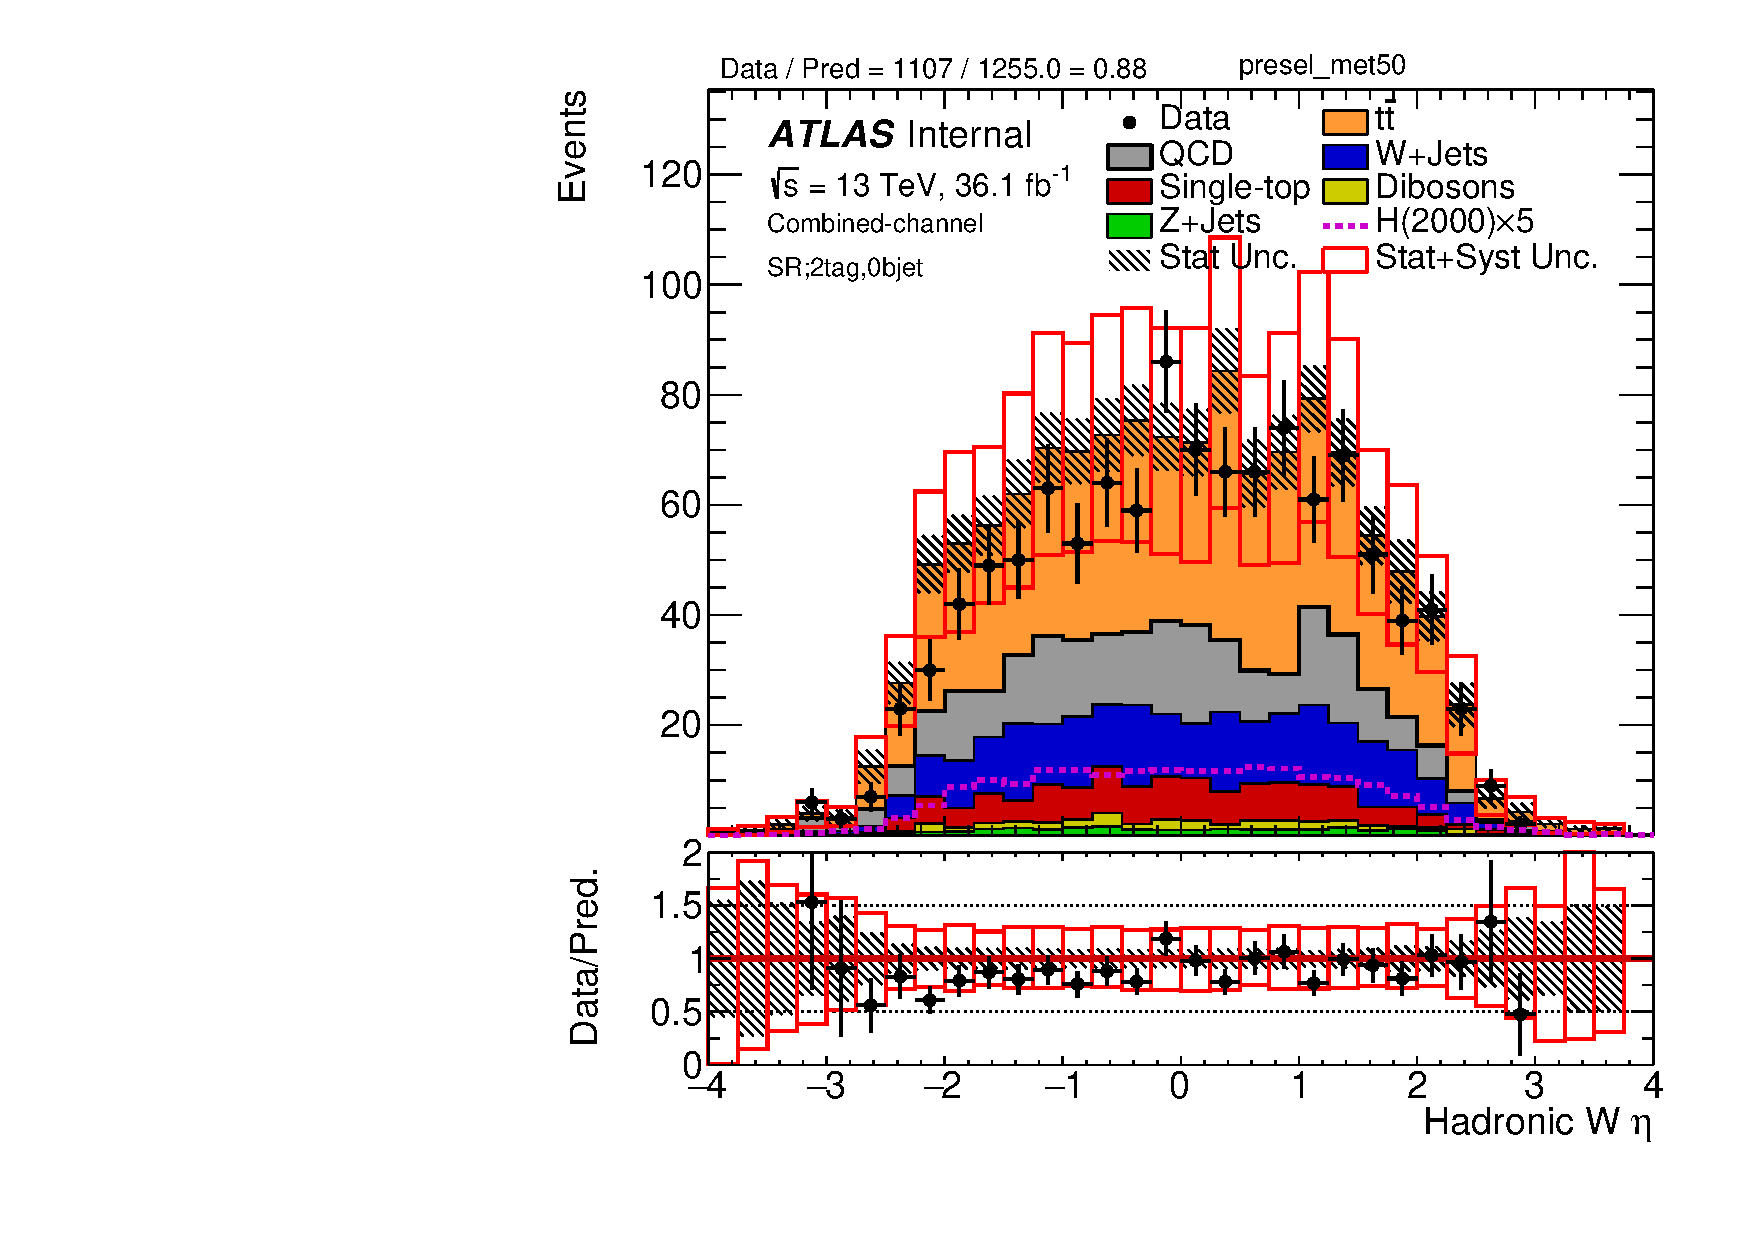
\includegraphics[scale=0.33]{./figures/boosted/PlotsInMbbSR/Unblinded/DataMC_2tag_0bjet_SR_lepton_presel_met50_WhadEta}
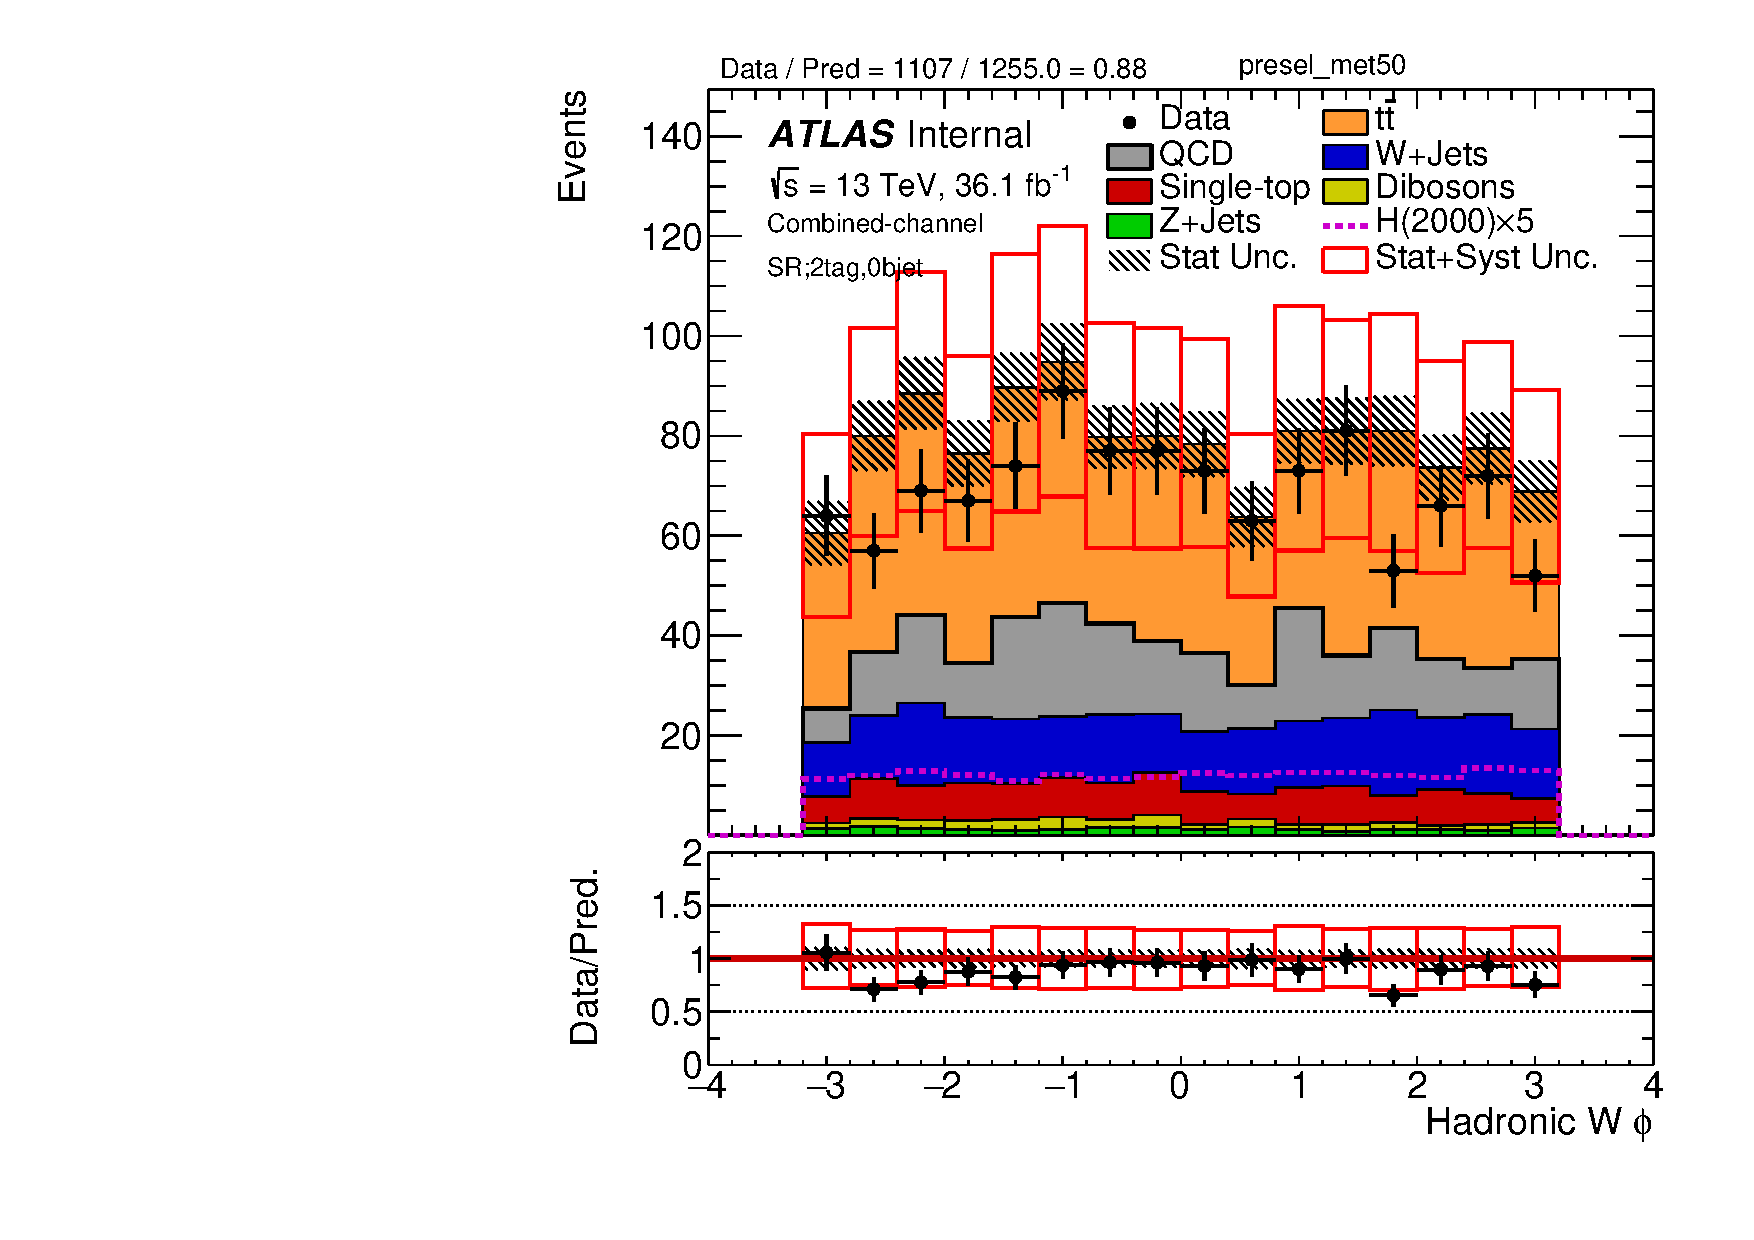
\includegraphics[scale=0.33]{./figures/boosted/PlotsInMbbSR/Unblinded/DataMC_2tag_0bjet_SR_lepton_presel_met50_WhadPhi}
\caption{Kinematic distributions of the reconstructed $W \to q\bar{q}$ system in the signal region (SR).}
\label{fig:boosted_SR_whad}
\end{center}
\end{figure}

\begin{figure}[!h]
\begin{center}
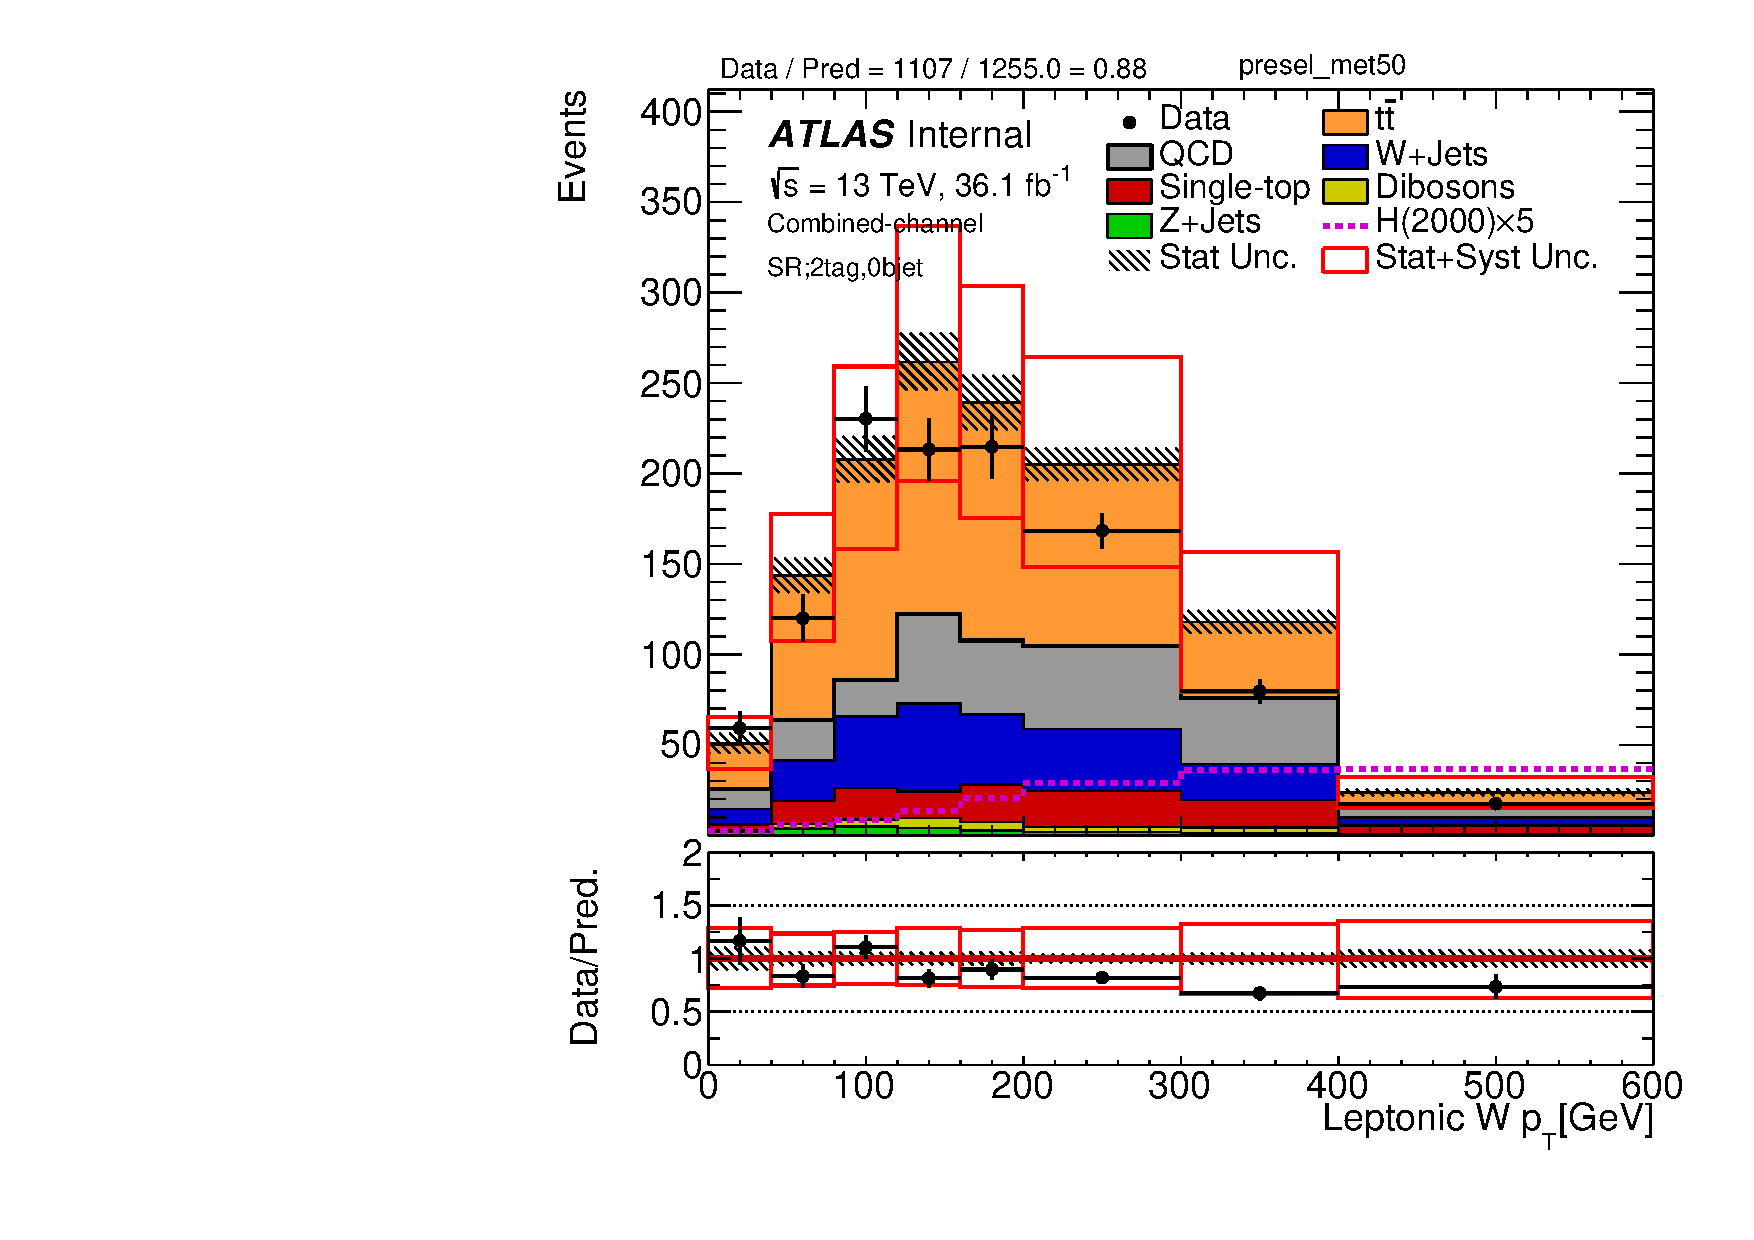
\includegraphics[scale=0.33]{./figures/boosted/PlotsInMbbSR/Unblinded/DataMC_2tag_0bjet_SR_lepton_presel_met50_WlepPt}
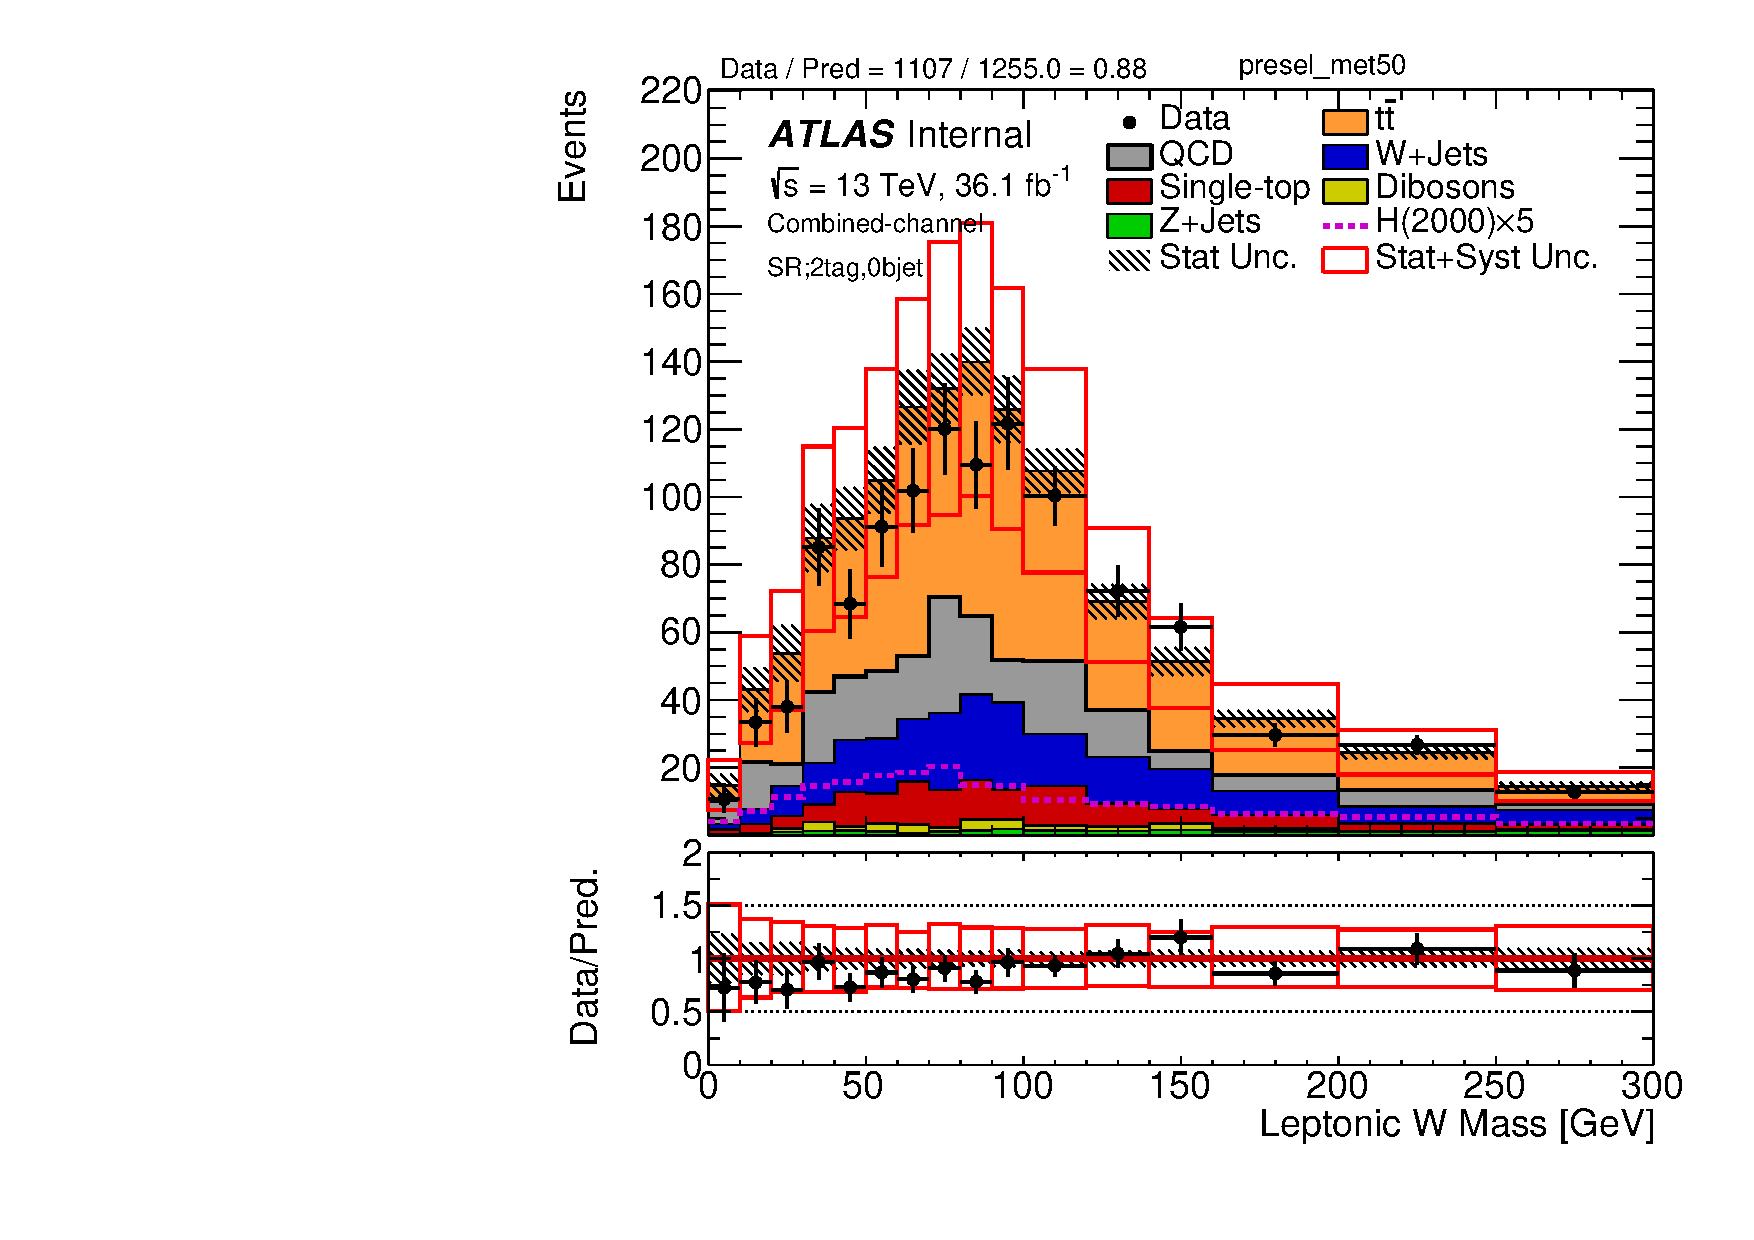
\includegraphics[scale=0.33]{./figures/boosted/PlotsInMbbSR/Unblinded/DataMC_2tag_0bjet_SR_lepton_presel_met50_WlepMass} \\
\par\medskip
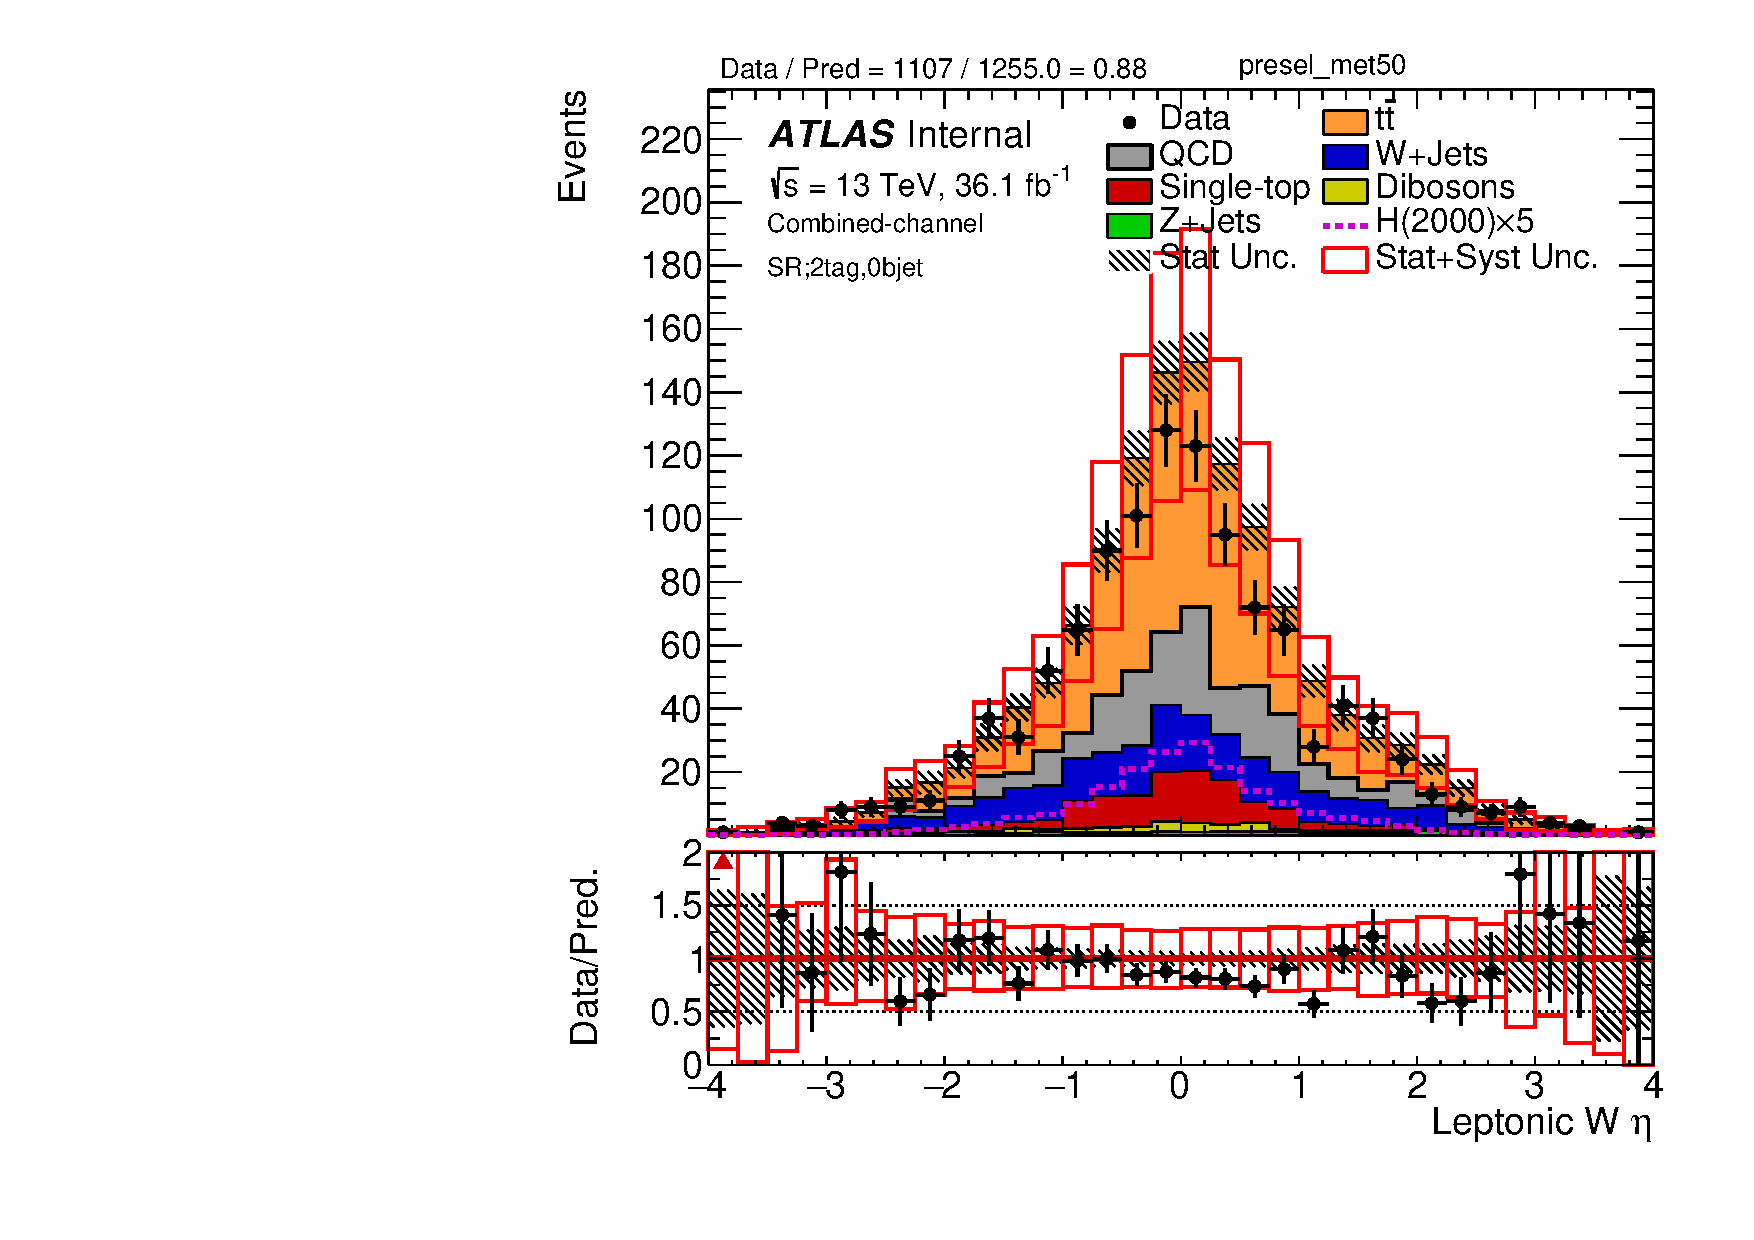
\includegraphics[scale=0.33]{./figures/boosted/PlotsInMbbSR/Unblinded/DataMC_2tag_0bjet_SR_lepton_presel_met50_WlepEta} 
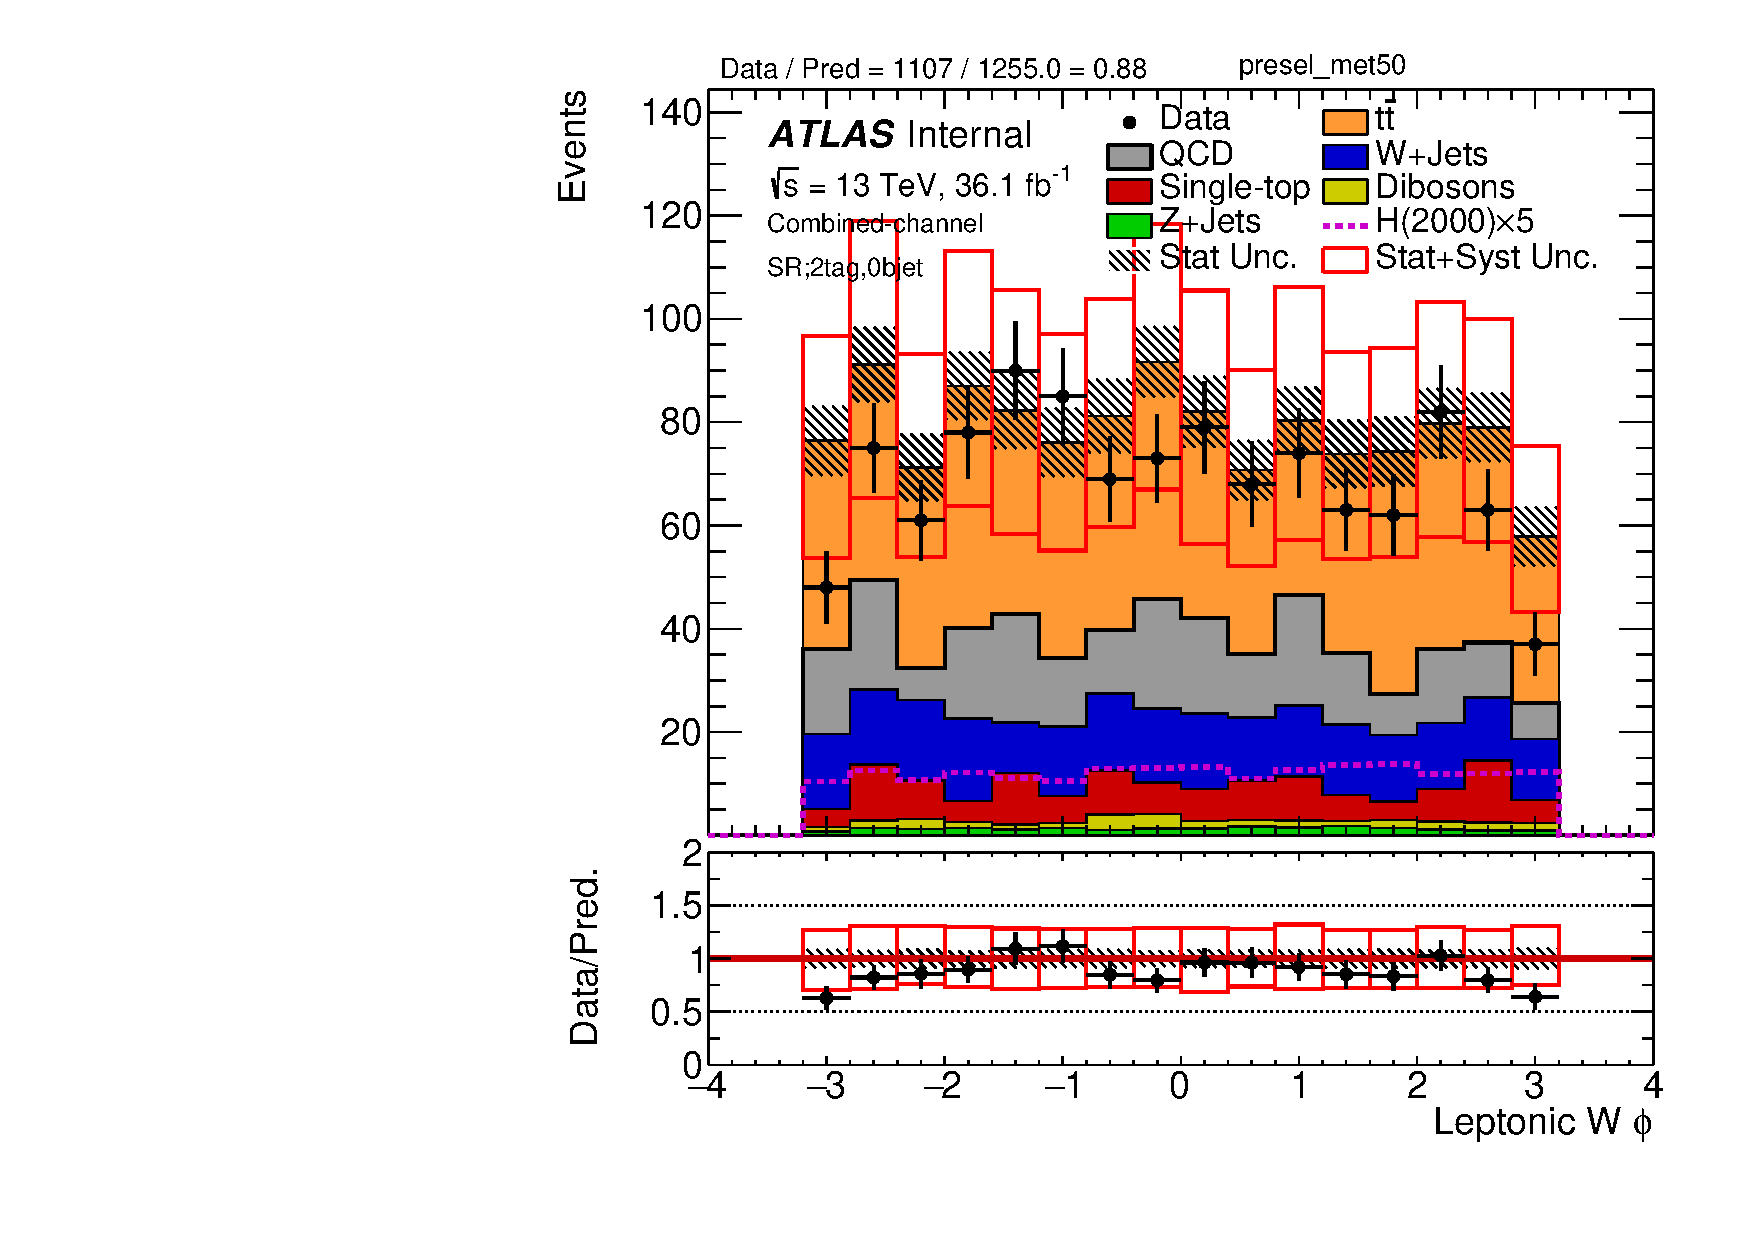
\includegraphics[scale=0.33]{./figures/boosted/PlotsInMbbSR/Unblinded/DataMC_2tag_0bjet_SR_lepton_presel_met50_WlepPhi}
\caption{Kinematic distributions of the reconstructed $W \to l\nu$ system in the signal region (SR).}
\label{fig:boosted_SR_wlep}
\end{center}
\end{figure}

\begin{figure}[!h]
\begin{center}
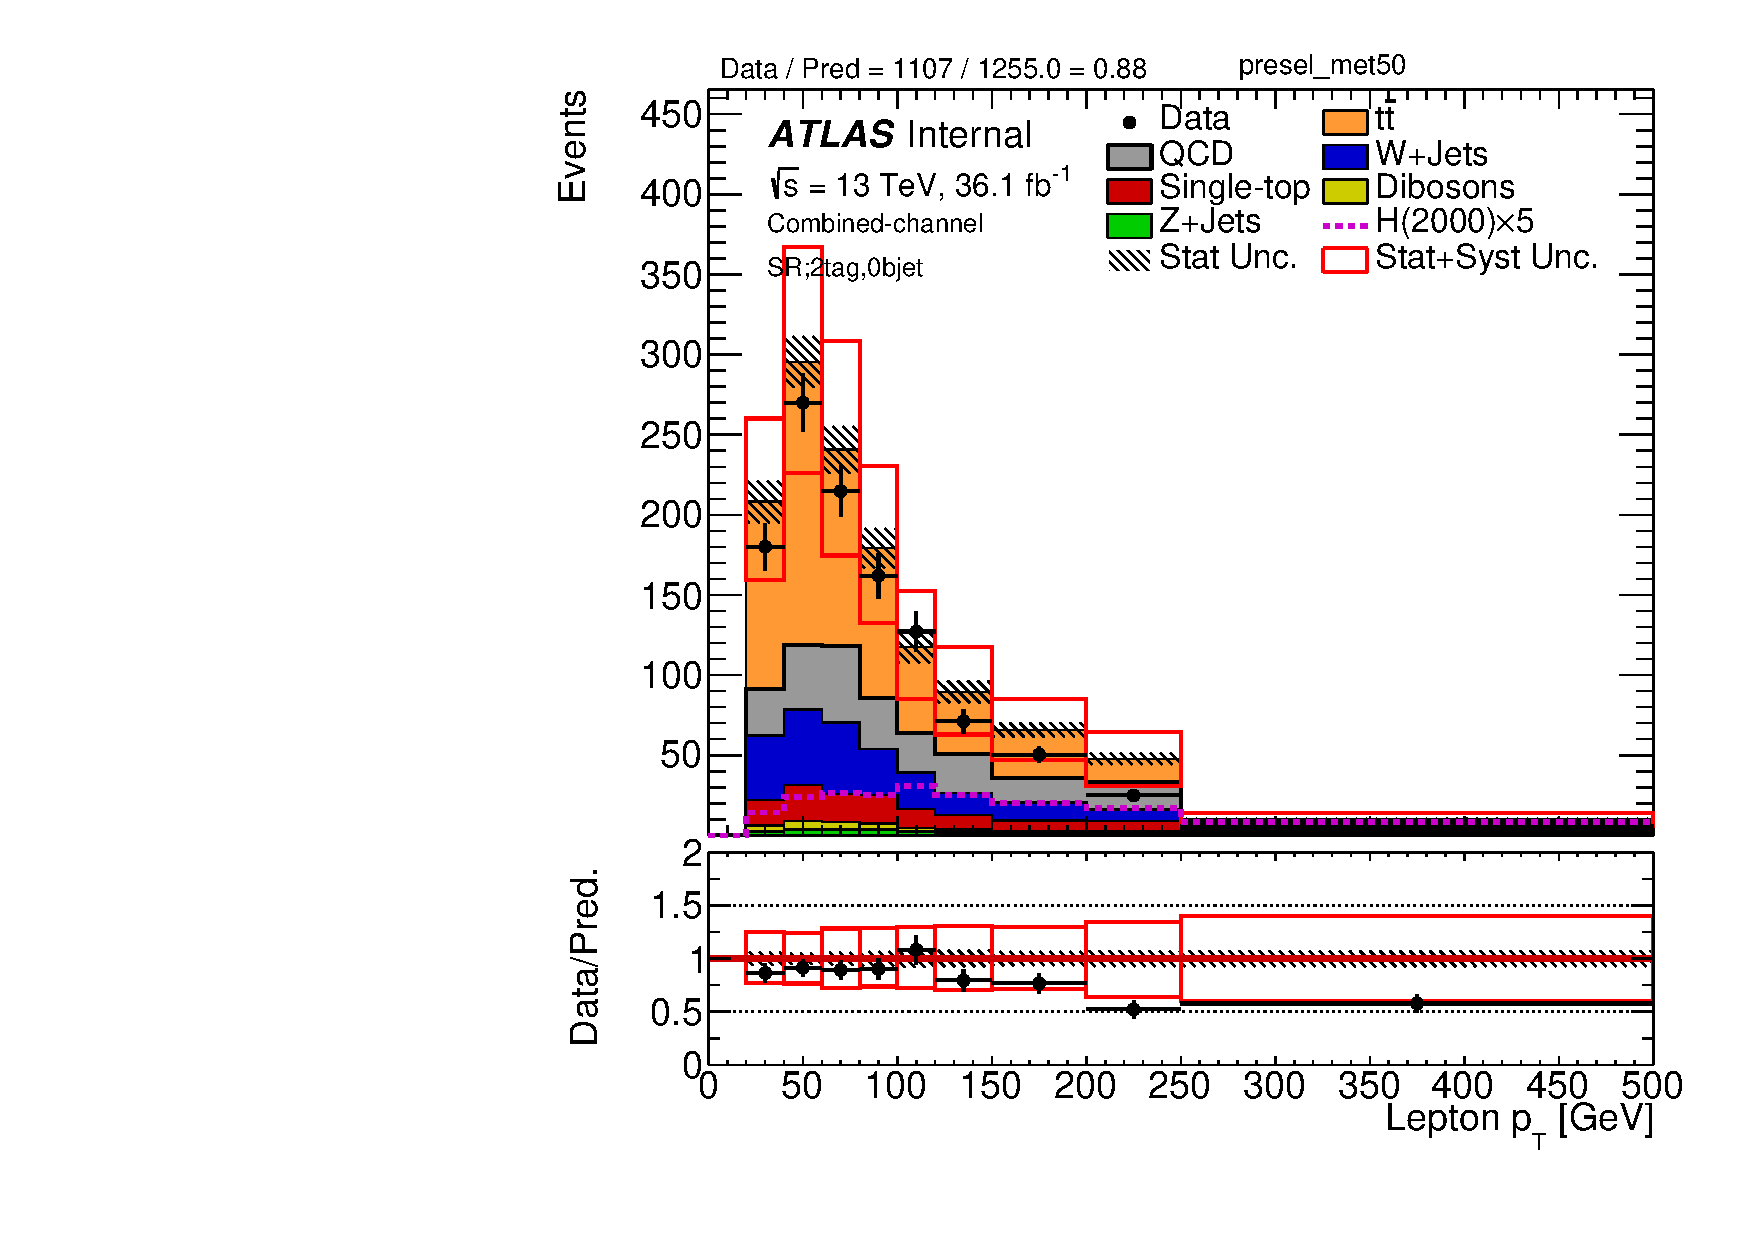
\includegraphics[scale=0.33]{./figures/boosted/PlotsInMbbSR/Unblinded/DataMC_2tag_0bjet_SR_lepton_presel_met50_LepPt}
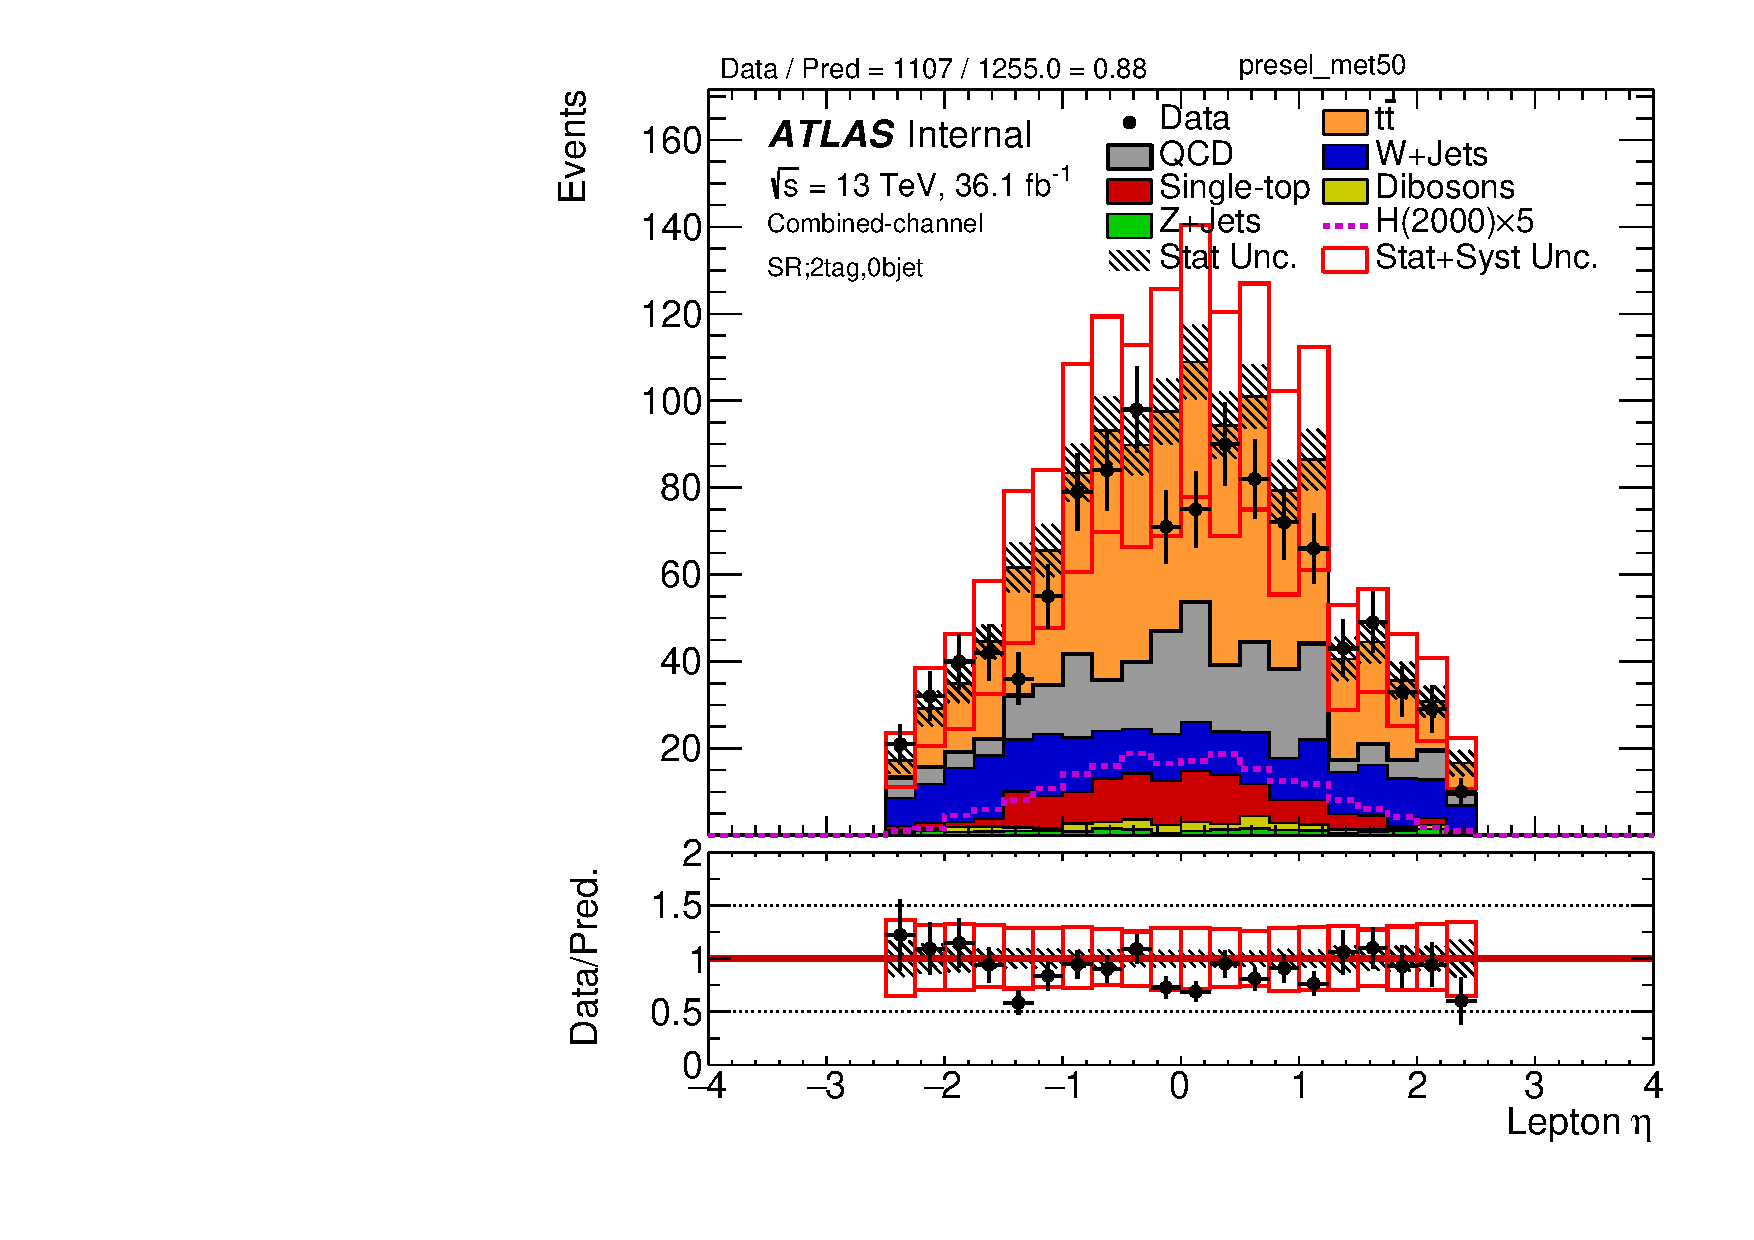
\includegraphics[scale=0.33]{./figures/boosted/PlotsInMbbSR/Unblinded/DataMC_2tag_0bjet_SR_lepton_presel_met50_LepEta}\\
\par\medskip
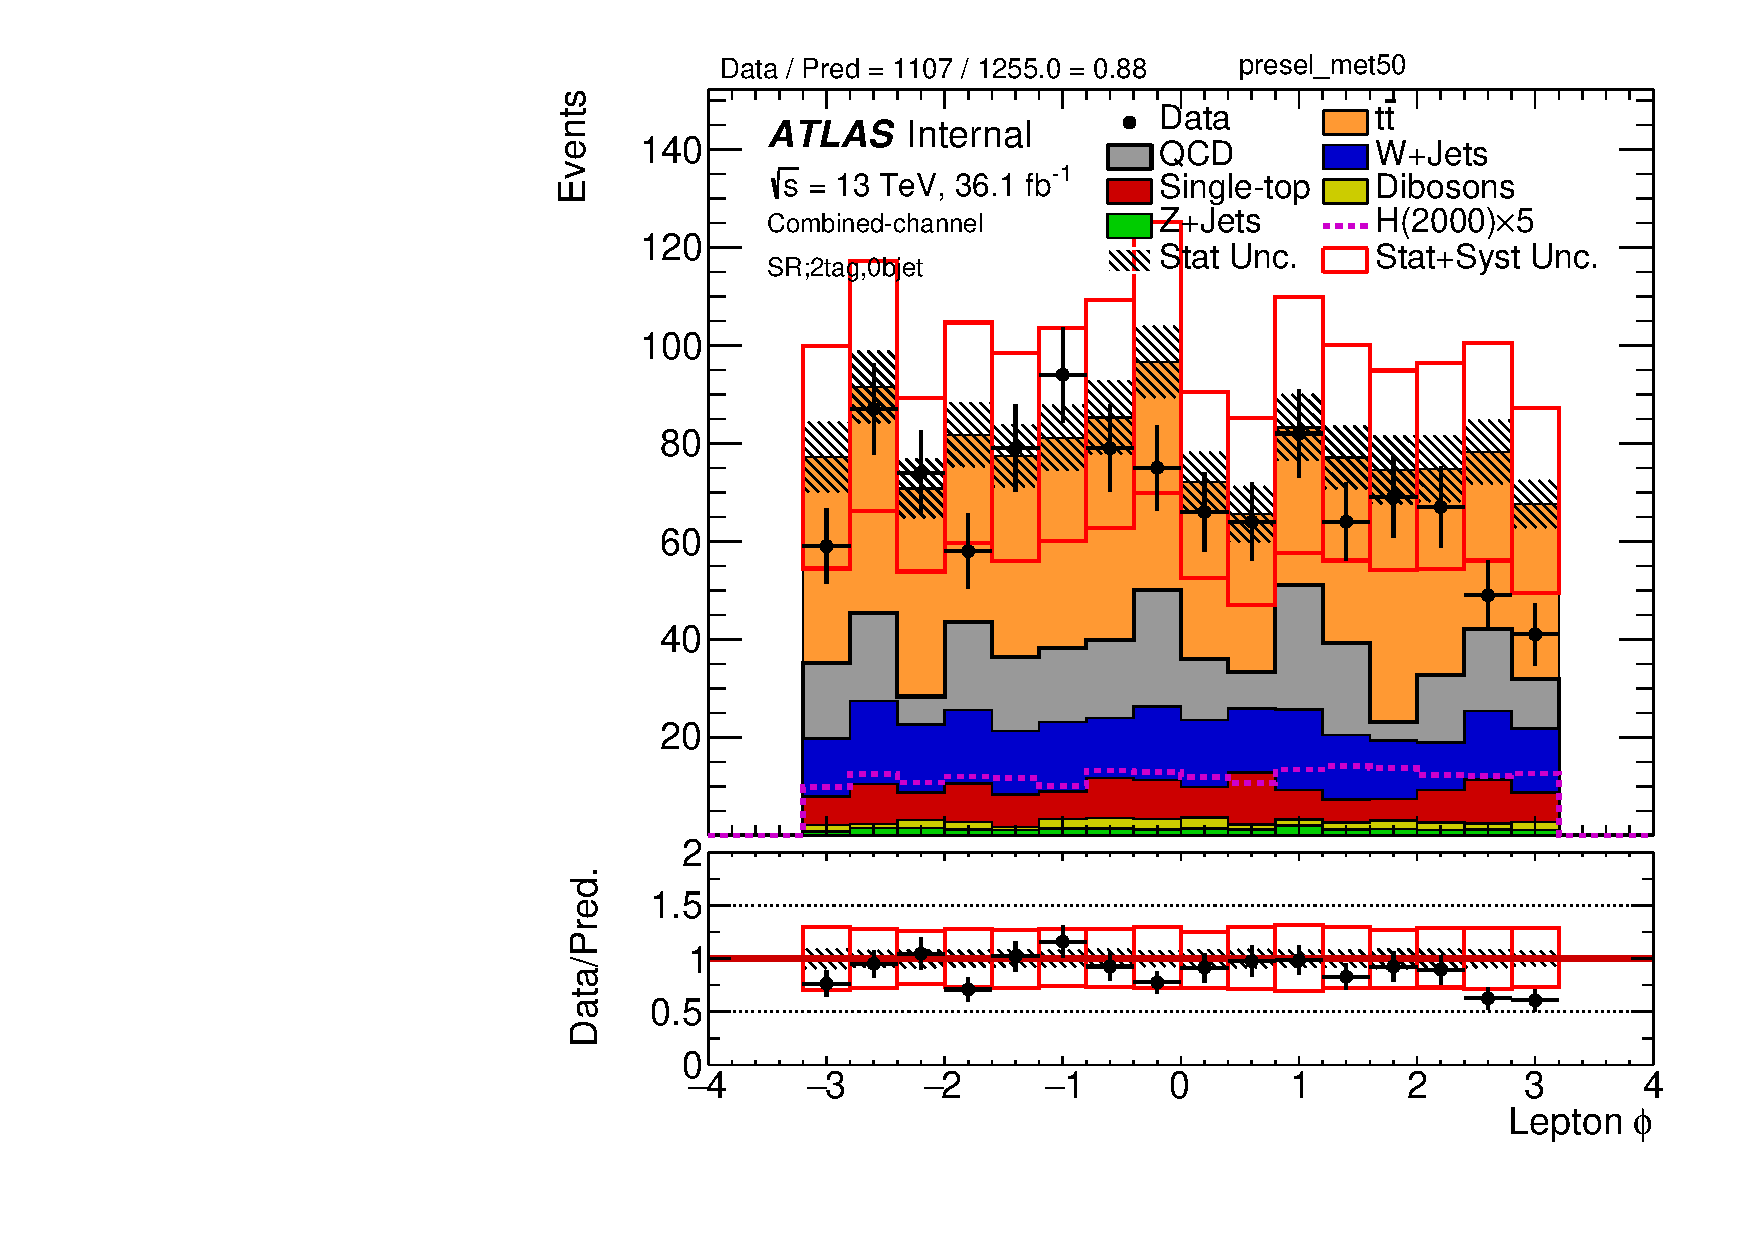
\includegraphics[scale=0.33]{./figures/boosted/PlotsInMbbSR/Unblinded/DataMC_2tag_0bjet_SR_lepton_presel_met50_LepPhi}
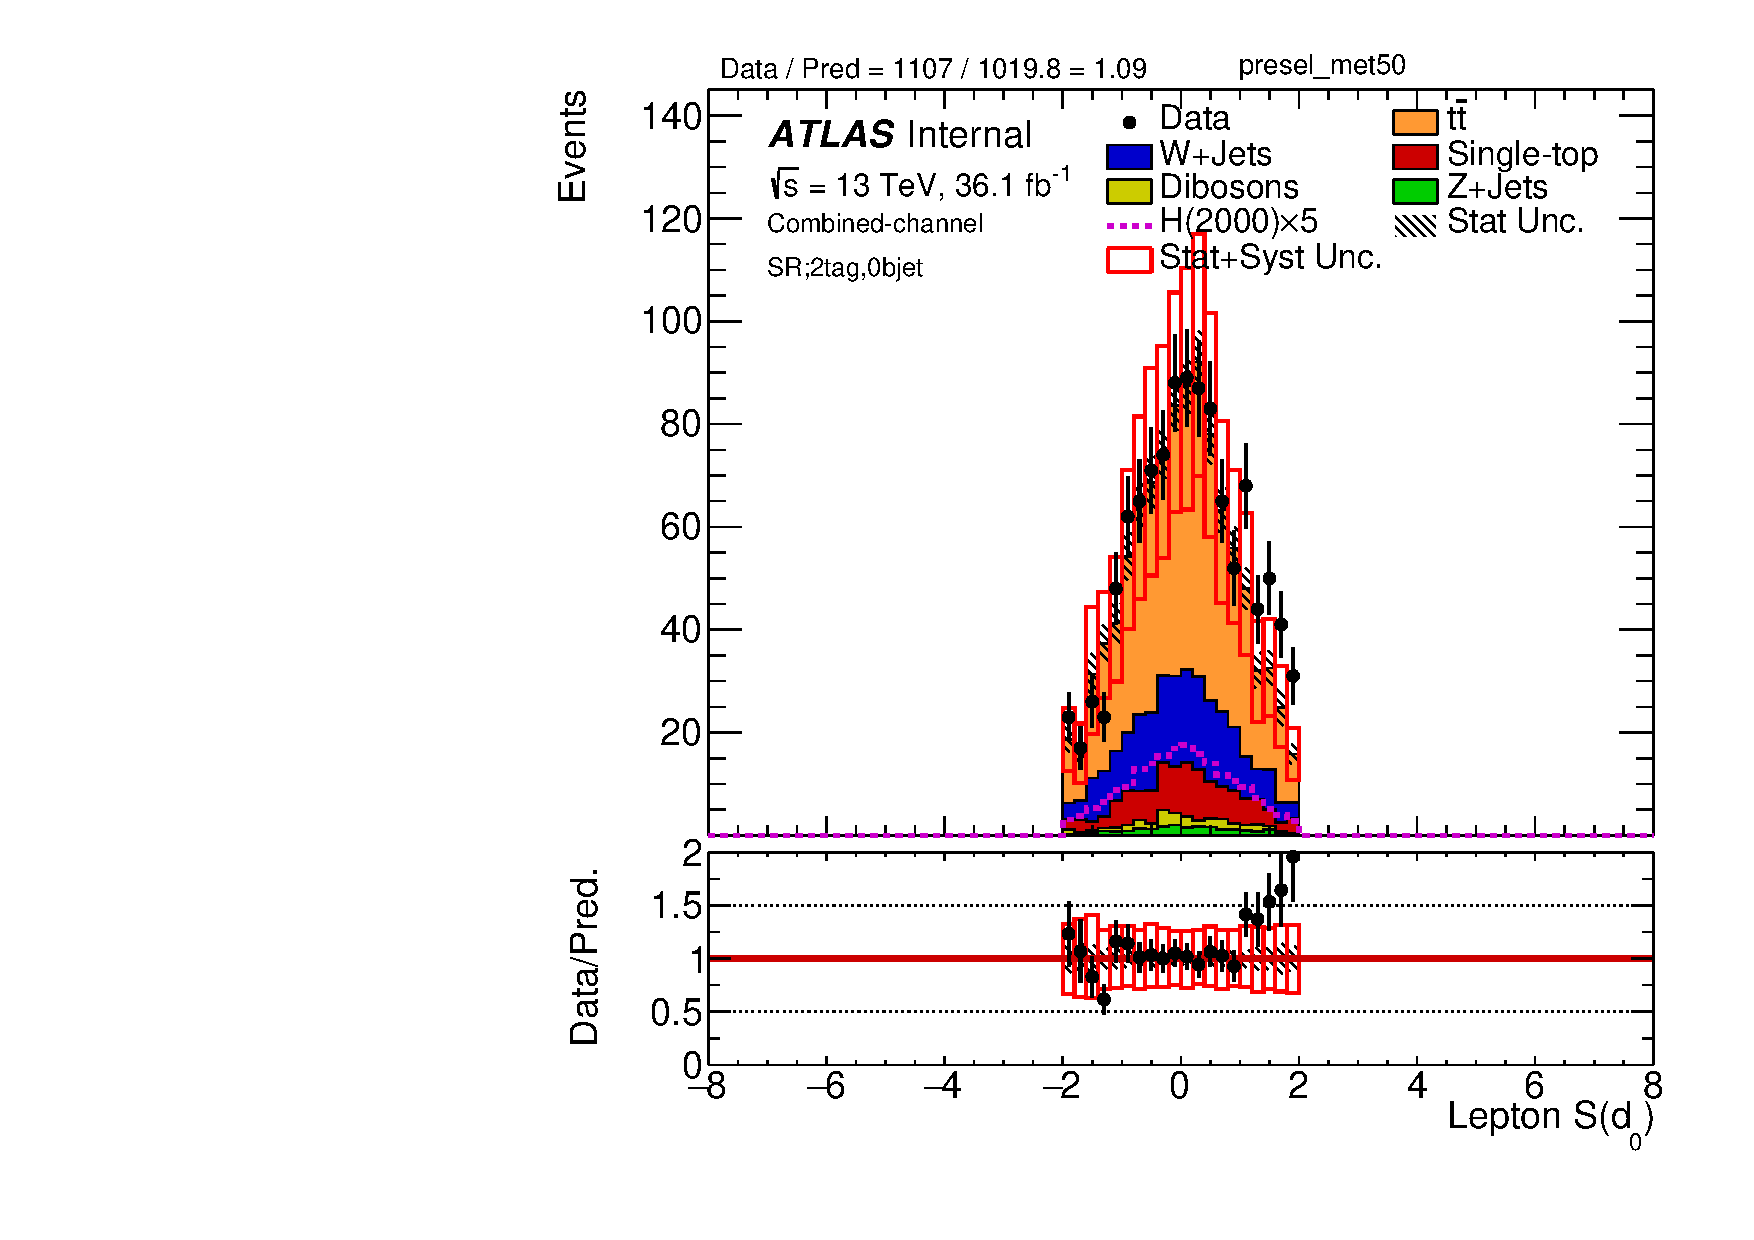
\includegraphics[scale=0.33]{./figures/boosted/PlotsInMbbSR/Unblinded/DataMC_2tag_0bjet_SR_lepton_presel_met50_Lep_d0sigL}
\caption{Kinematic distributions of the selected lepton in the signal region (SR).}
\label{fig:boosted_SR_lepton}
\end{center}
\end{figure}


\begin{figure}[!ht]
\begin{center}
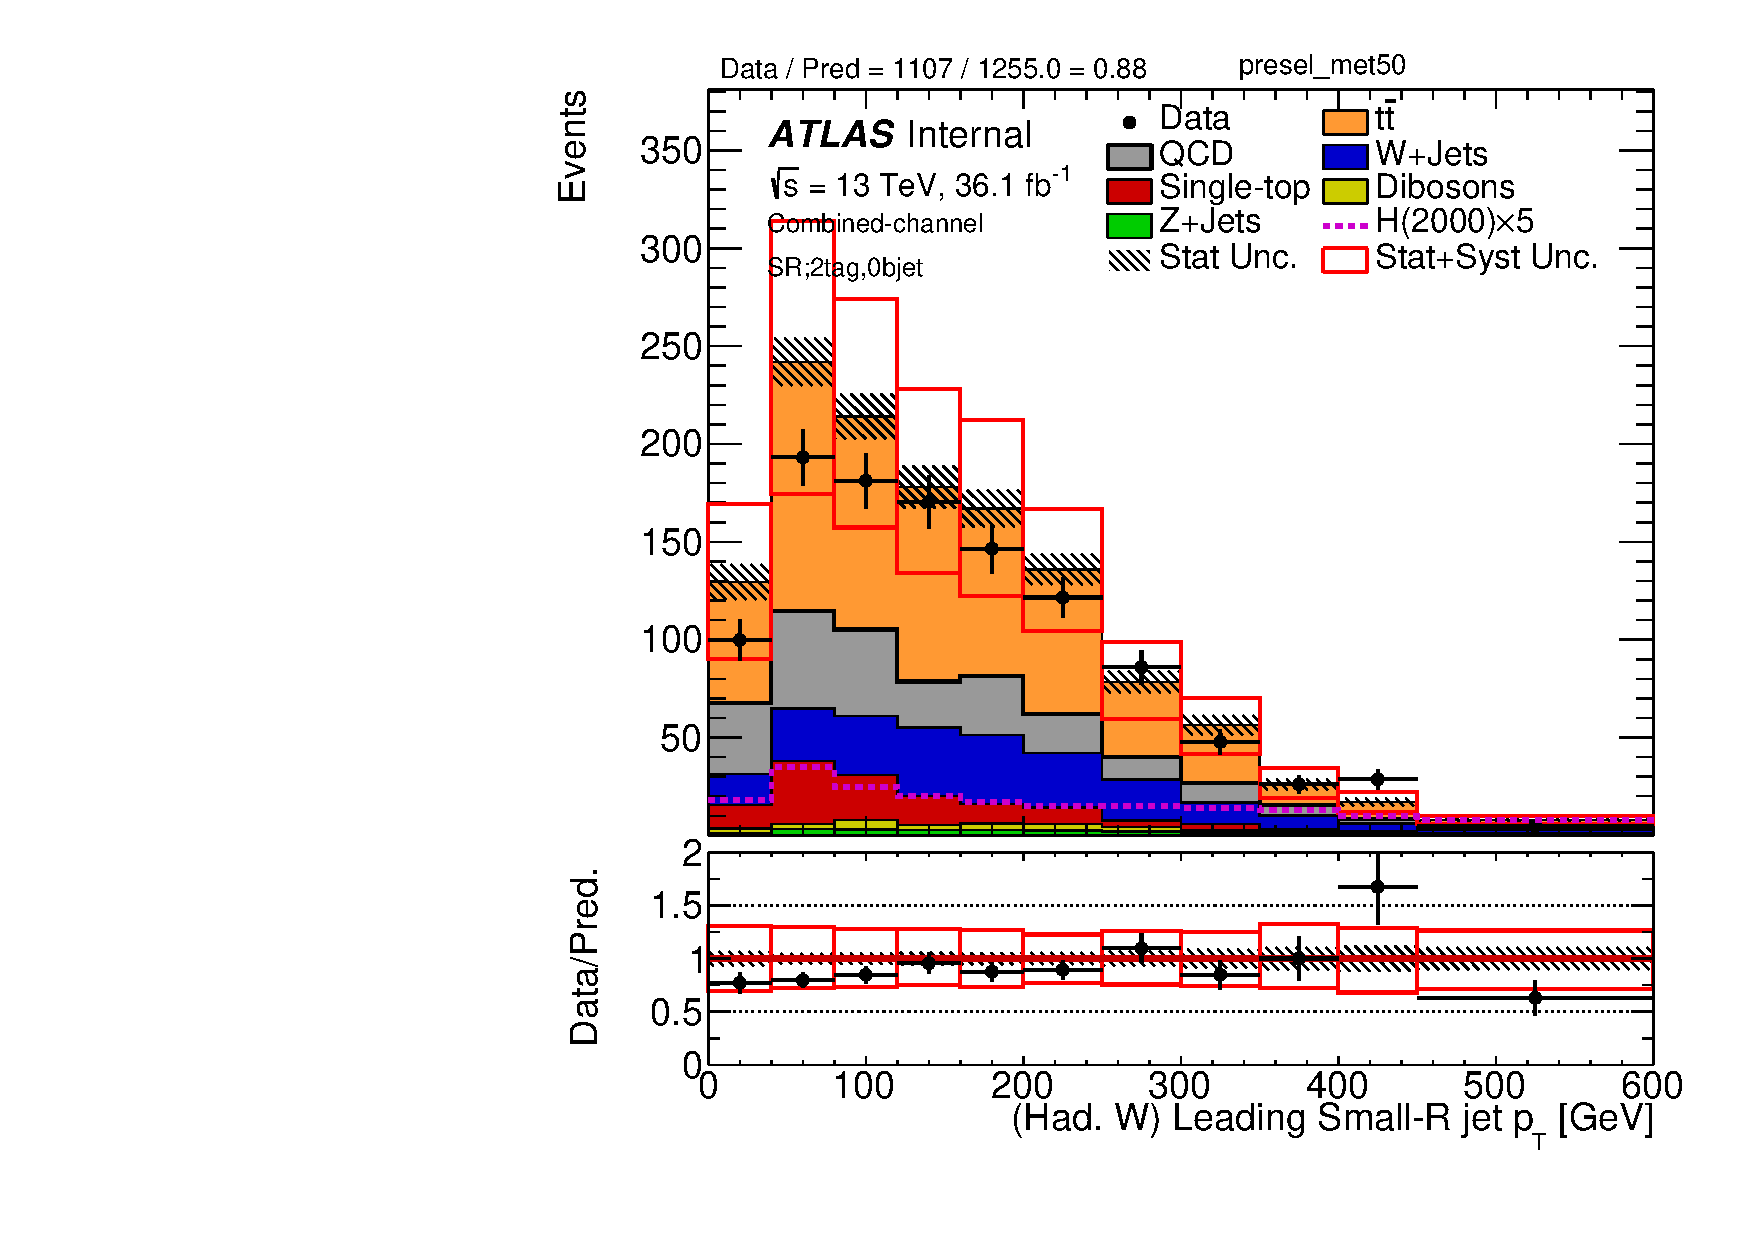
\includegraphics[scale=0.33]{./figures/boosted/PlotsInMbbSR/Unblinded/DataMC_2tag_0bjet_SR_lepton_presel_met50_LightJet1Pt}
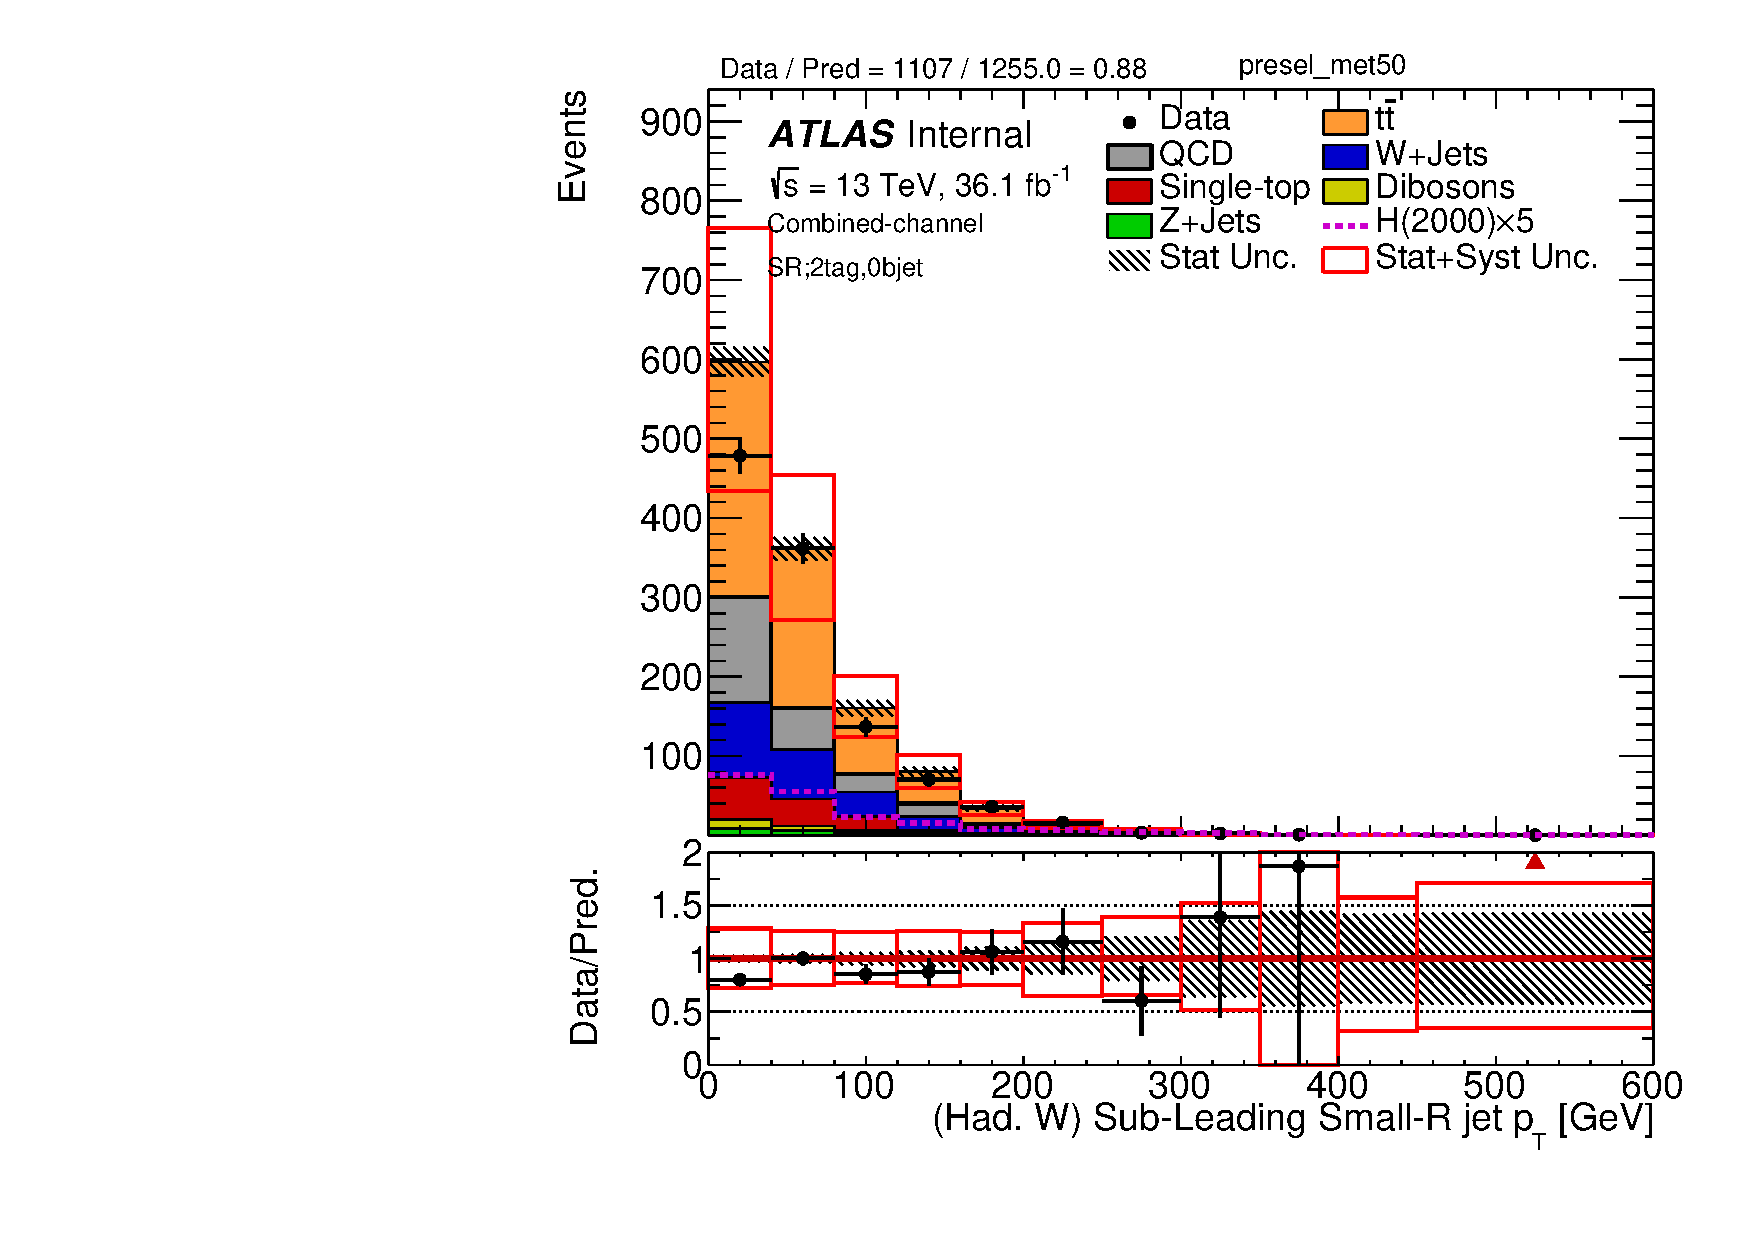
\includegraphics[scale=0.33]{./figures/boosted/PlotsInMbbSR/Unblinded/DataMC_2tag_0bjet_SR_lepton_presel_met50_LightJet2Pt}\\
\par\medskip
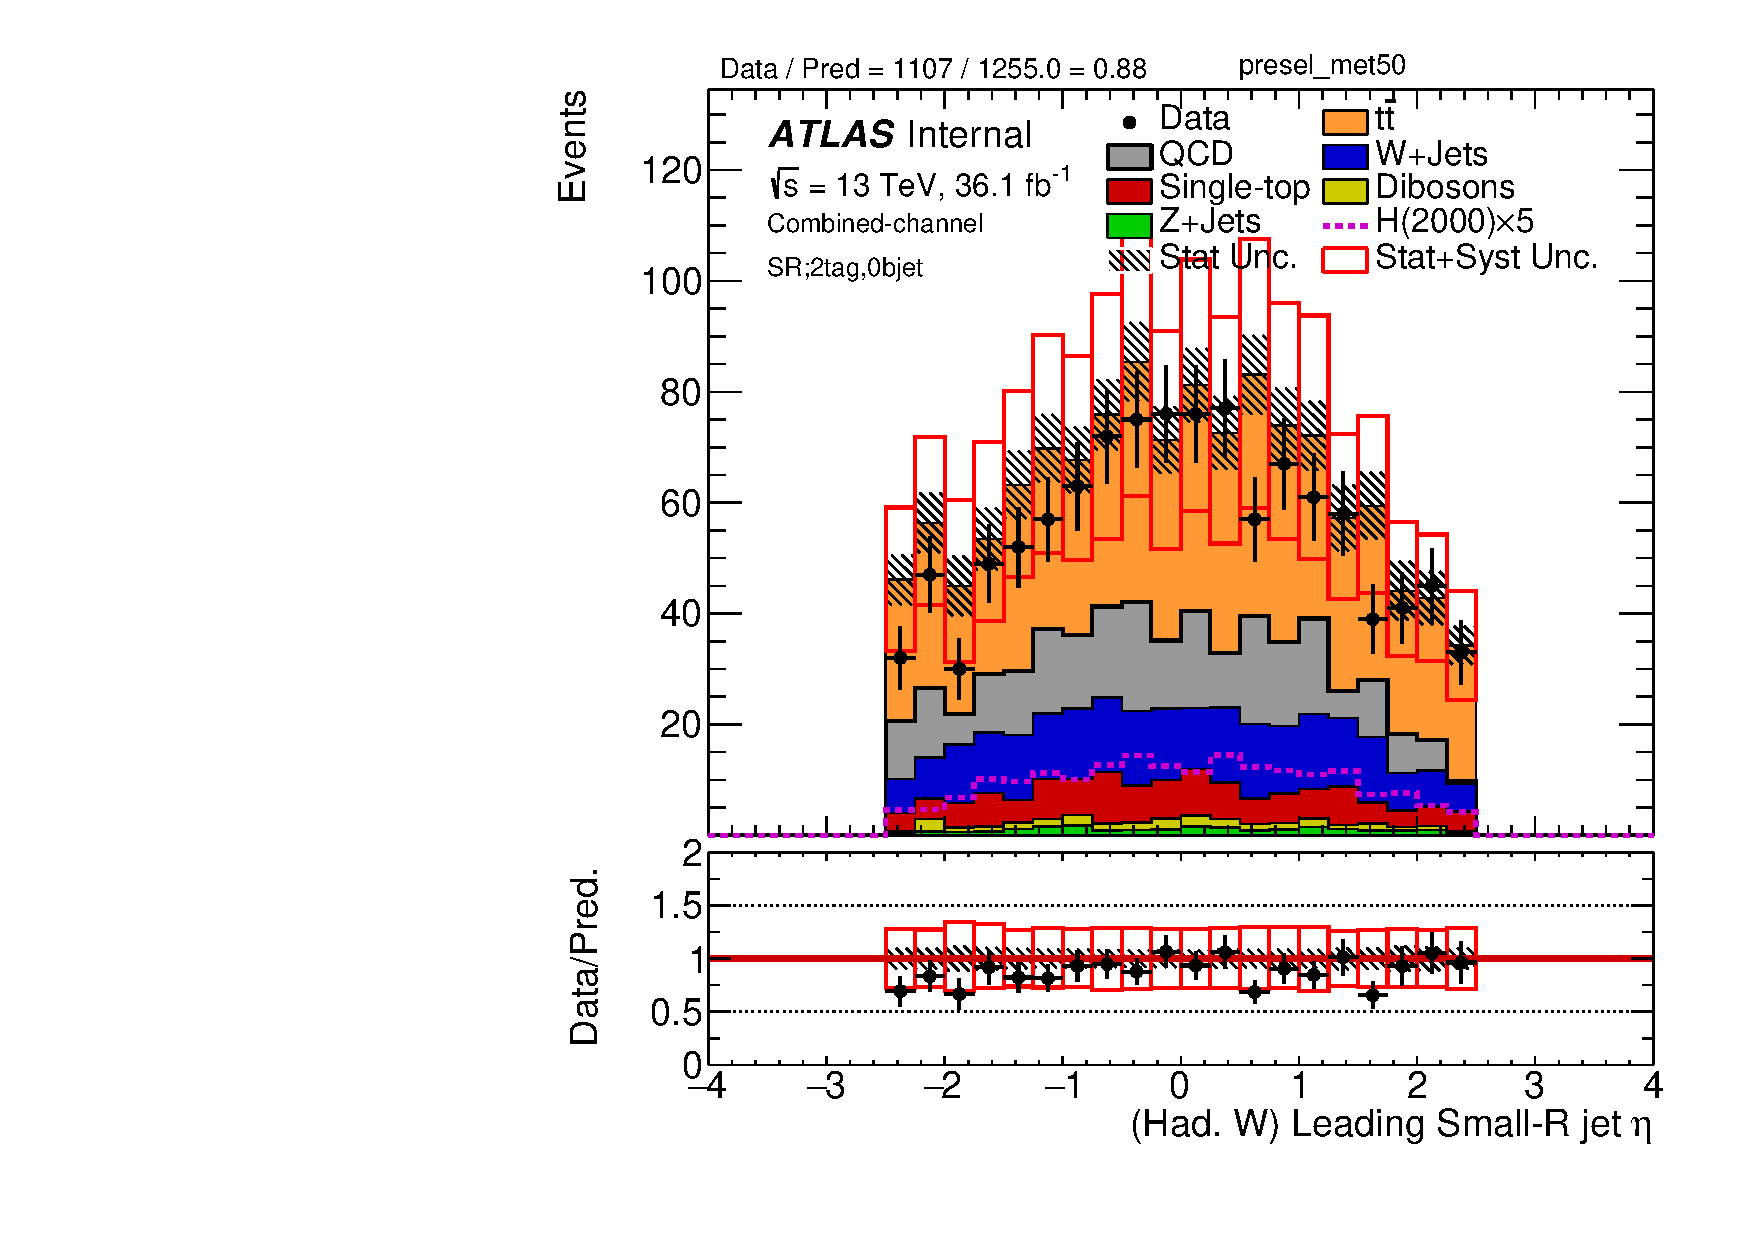
\includegraphics[scale=0.33]{./figures/boosted/PlotsInMbbSR/Unblinded/DataMC_2tag_0bjet_SR_lepton_presel_met50_LightJet1Eta}
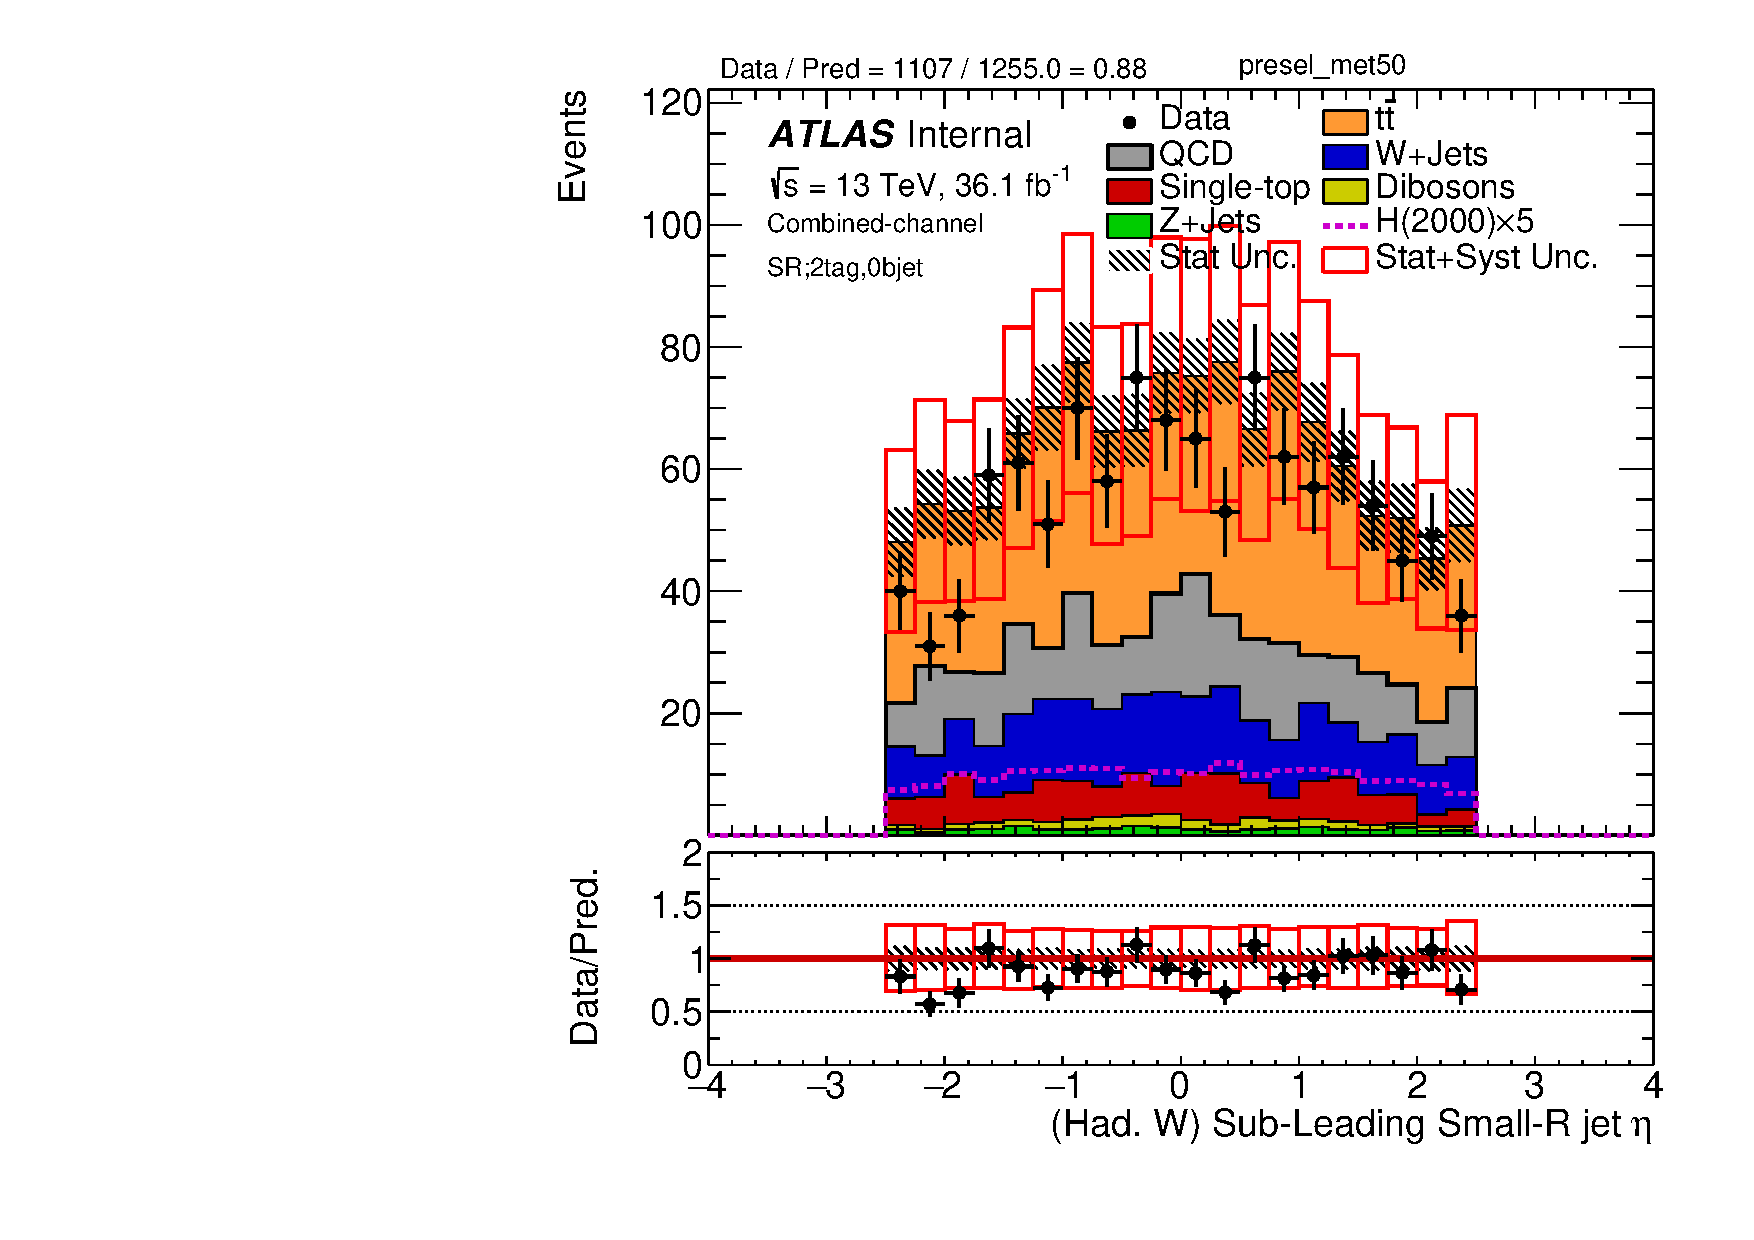
\includegraphics[scale=0.33]{./figures/boosted/PlotsInMbbSR/Unblinded/DataMC_2tag_0bjet_SR_lepton_presel_met50_LightJet2Eta}\\
\par\medskip
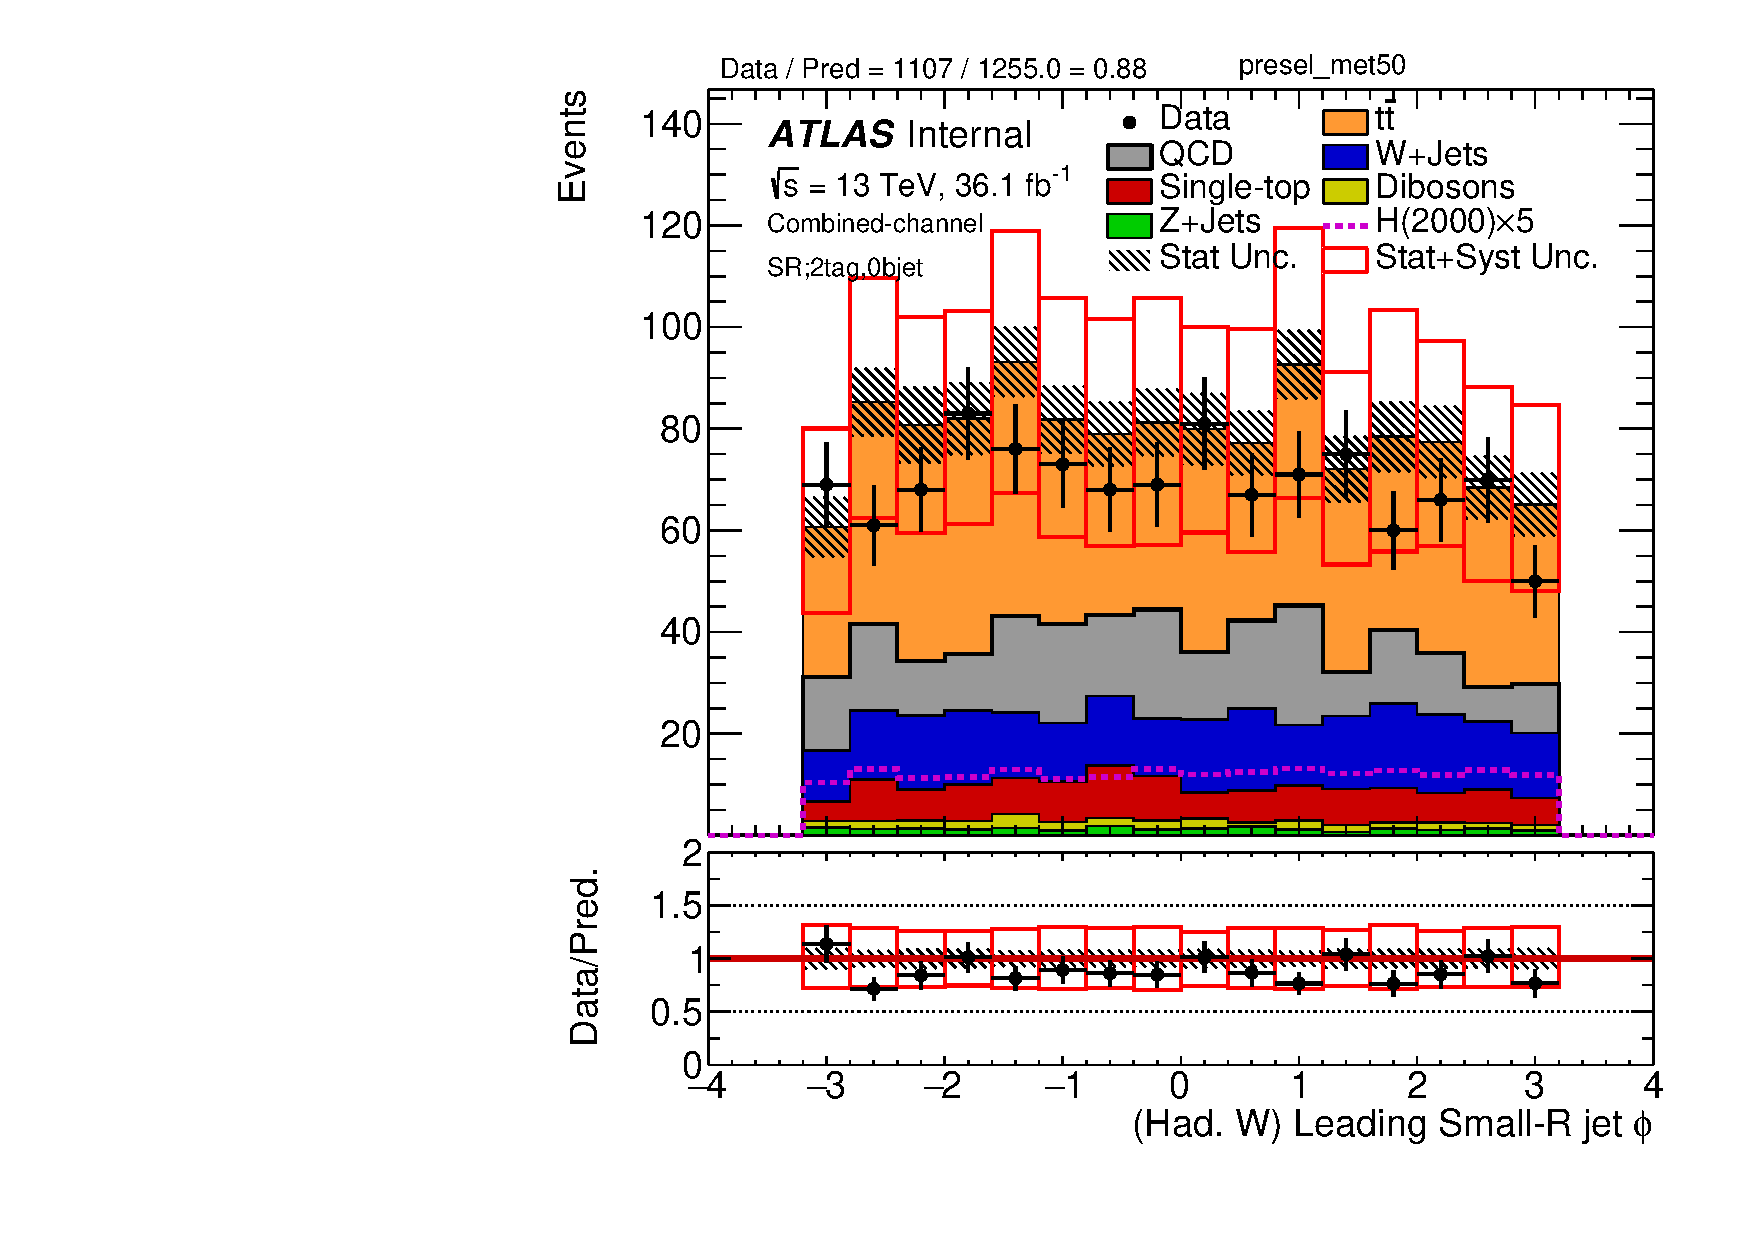
\includegraphics[scale=0.33]{./figures/boosted/PlotsInMbbSR/Unblinded/DataMC_2tag_0bjet_SR_lepton_presel_met50_LightJet1Phi}
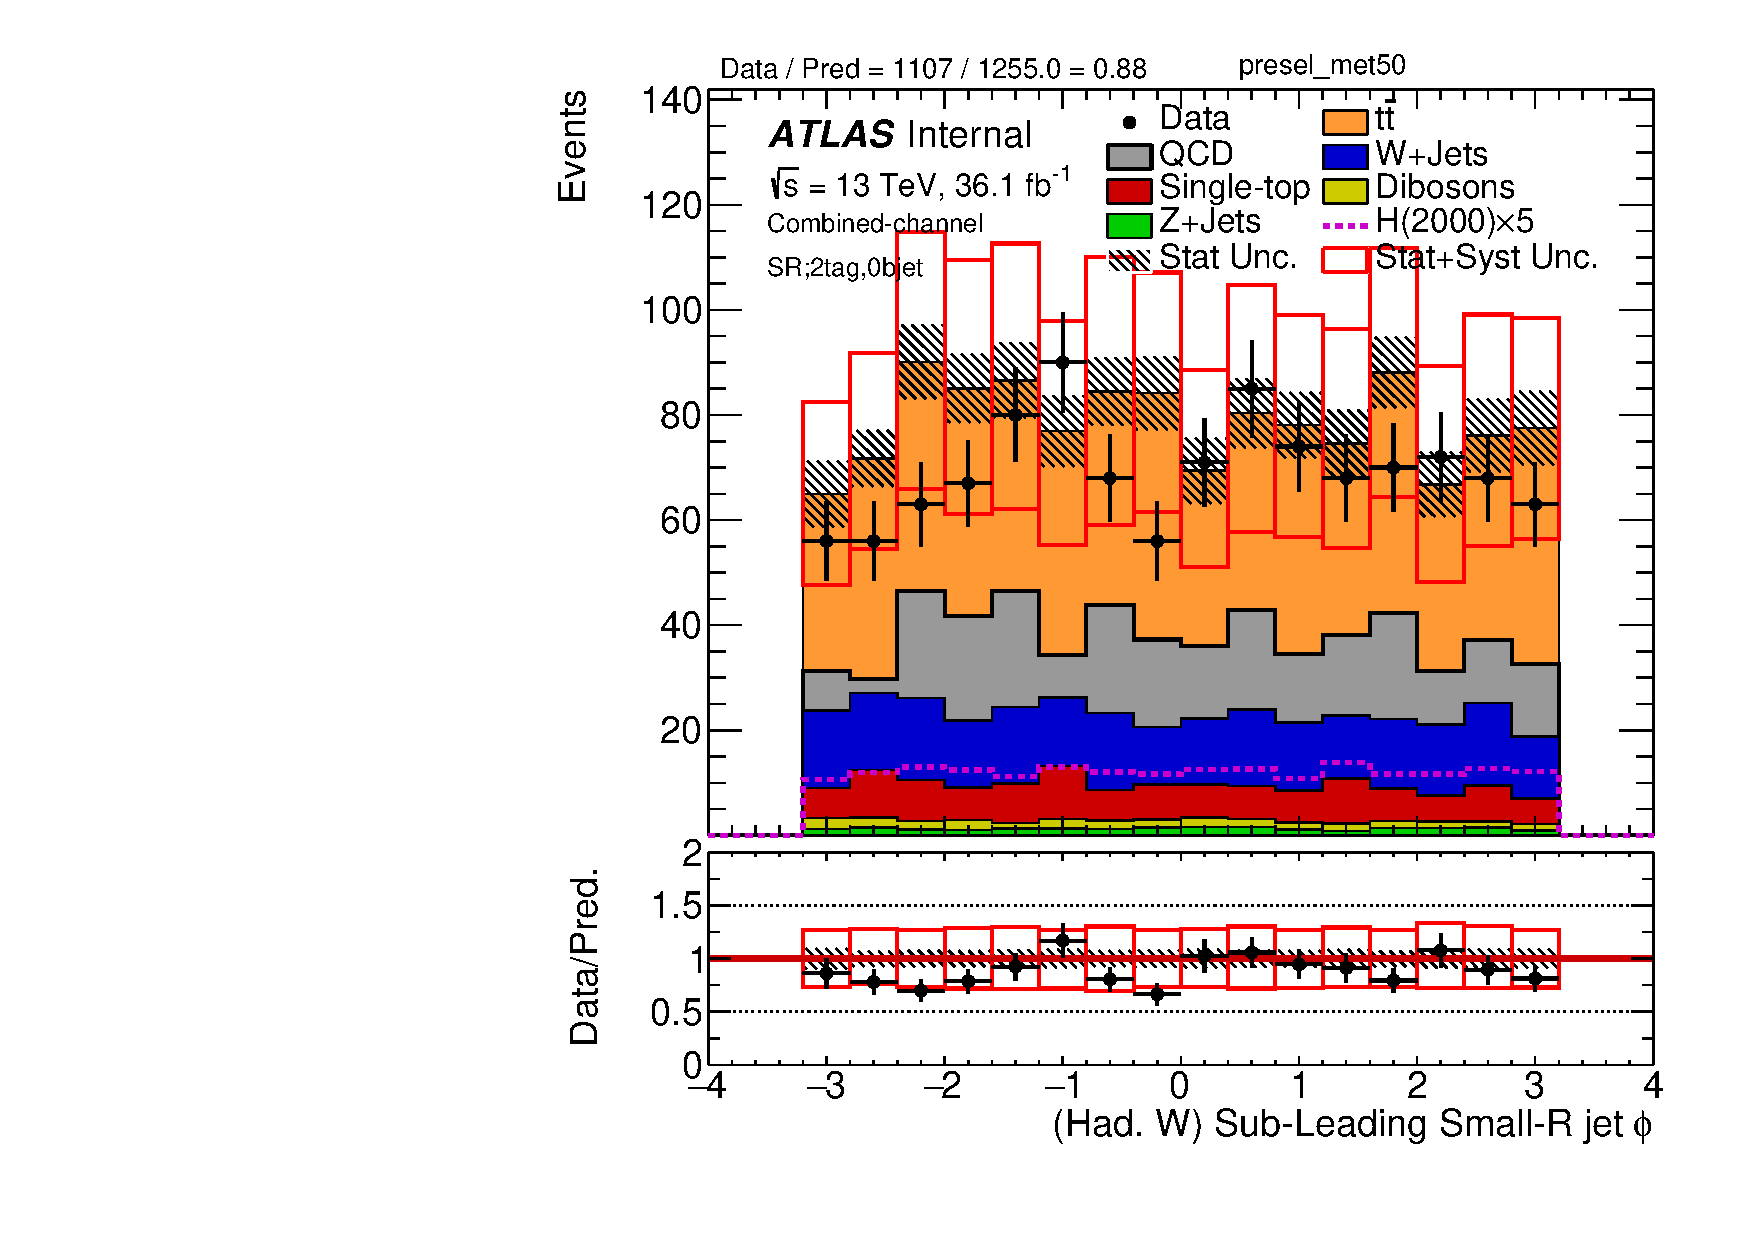
\includegraphics[scale=0.33]{./figures/boosted/PlotsInMbbSR/Unblinded/DataMC_2tag_0bjet_SR_lepton_presel_met50_LightJet2Phi}\\
\caption{Kinematic distributions of the leading and sub-leading small-$R$ jets (of the reconstructed hadronic W) 
in the signal region (SR).}
\label{fig:boosted_SR_whad_jets}
\end{center}
\end{figure}

\begin{figure}[!h]
\begin{center}
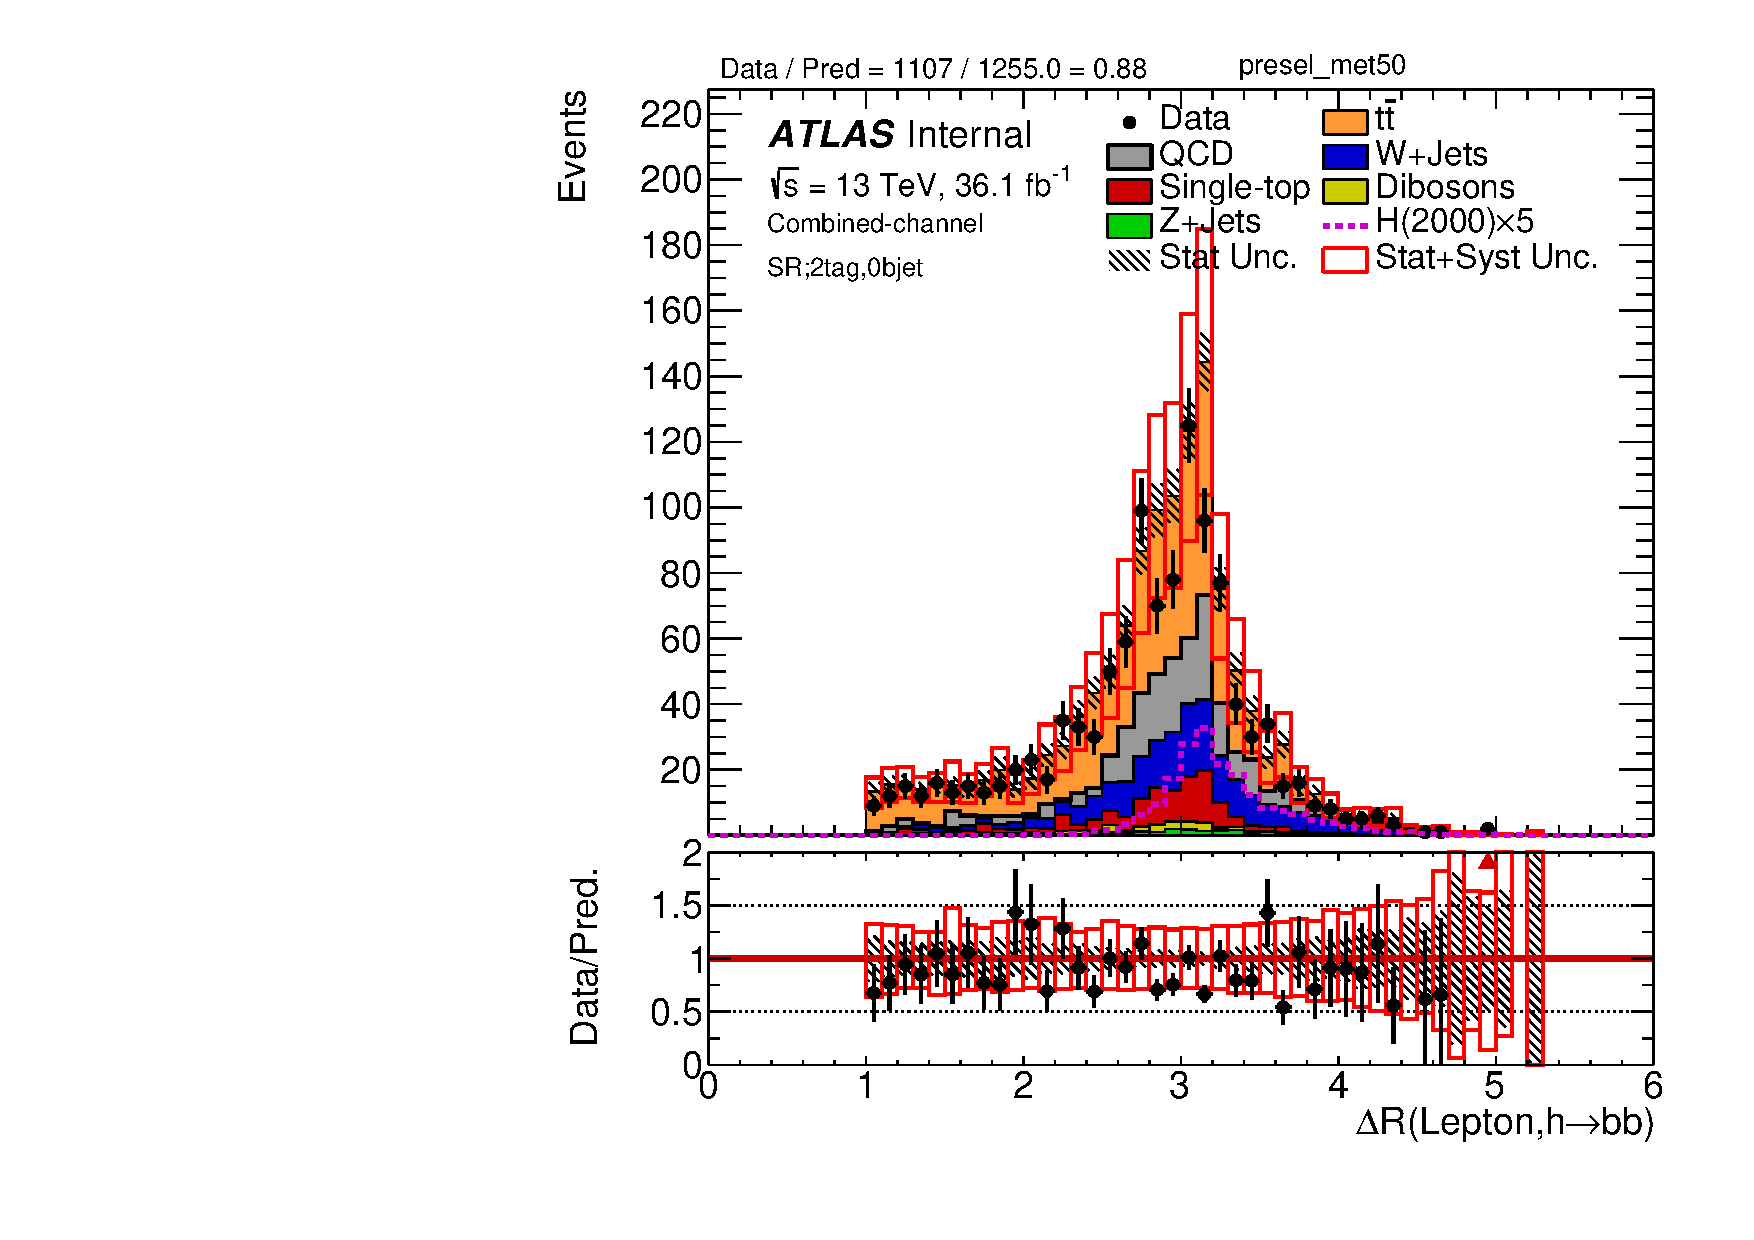
\includegraphics[scale=0.33]{./figures/boosted/PlotsInMbbSR/Unblinded/DataMC_2tag_0bjet_SR_lepton_presel_met50_drHbbLep}
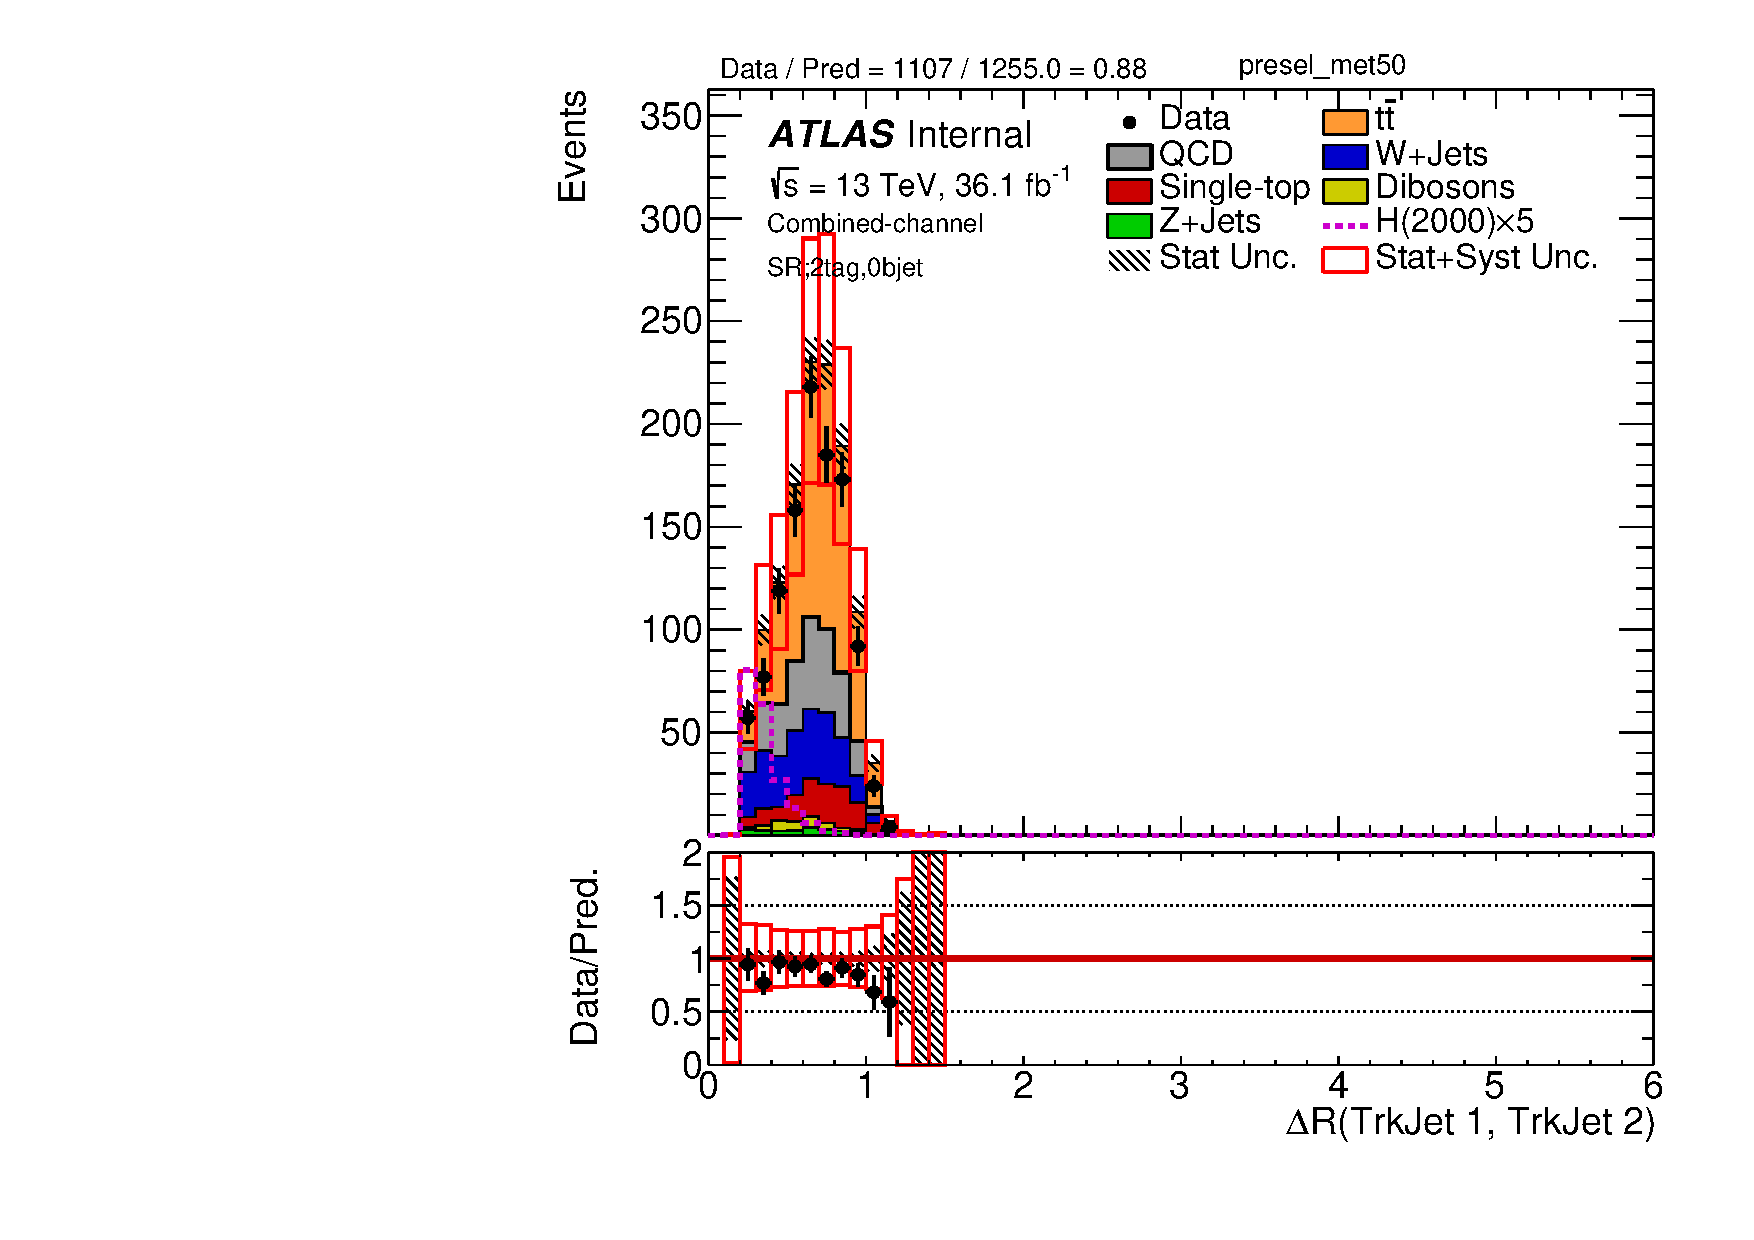
\includegraphics[scale=0.33]{./figures/boosted/PlotsInMbbSR/Unblinded/DataMC_2tag_0bjet_SR_lepton_presel_met50_drbtrkjet1btrkjet2} \\
\caption{$\Delta R$ distribution between the selected lepton and the large-$R$ jet and $\Delta R$ distribution between the track-jets inside
the large-$R$ jet in the signal region (SR).}
\label{fig:boosted_SR_dr}
\end{center}
\end{figure}
